\documentclass[twoside]{book}

% Packages required by doxygen
\usepackage{fixltx2e}
\usepackage{calc}
\usepackage{doxygen}
\usepackage[export]{adjustbox} % also loads graphicx
\usepackage{graphicx}
\usepackage[utf8]{inputenc}
\usepackage{makeidx}
\usepackage{multicol}
\usepackage{multirow}
\PassOptionsToPackage{warn}{textcomp}
\usepackage{textcomp}
\usepackage[nointegrals]{wasysym}
\usepackage[table]{xcolor}

% Font selection
\usepackage[T1]{fontenc}
\usepackage[scaled=.90]{helvet}
\usepackage{courier}
\usepackage{amssymb}
\usepackage{sectsty}
\renewcommand{\familydefault}{\sfdefault}
\allsectionsfont{%
  \fontseries{bc}\selectfont%
  \color{darkgray}%
}
\renewcommand{\DoxyLabelFont}{%
  \fontseries{bc}\selectfont%
  \color{darkgray}%
}
\newcommand{\+}{\discretionary{\mbox{\scriptsize$\hookleftarrow$}}{}{}}

% Page & text layout
\usepackage{geometry}
\geometry{%
  a4paper,%
  top=2.5cm,%
  bottom=2.5cm,%
  left=2.5cm,%
  right=2.5cm%
}
\tolerance=750
\hfuzz=15pt
\hbadness=750
\setlength{\emergencystretch}{15pt}
\setlength{\parindent}{0cm}
\setlength{\parskip}{3ex plus 2ex minus 2ex}
\makeatletter
\renewcommand{\paragraph}{%
  \@startsection{paragraph}{4}{0ex}{-1.0ex}{1.0ex}{%
    \normalfont\normalsize\bfseries\SS@parafont%
  }%
}
\renewcommand{\subparagraph}{%
  \@startsection{subparagraph}{5}{0ex}{-1.0ex}{1.0ex}{%
    \normalfont\normalsize\bfseries\SS@subparafont%
  }%
}
\makeatother

% Headers & footers
\usepackage{fancyhdr}
\pagestyle{fancyplain}
\fancyhead[LE]{\fancyplain{}{\bfseries\thepage}}
\fancyhead[CE]{\fancyplain{}{}}
\fancyhead[RE]{\fancyplain{}{\bfseries\leftmark}}
\fancyhead[LO]{\fancyplain{}{\bfseries\rightmark}}
\fancyhead[CO]{\fancyplain{}{}}
\fancyhead[RO]{\fancyplain{}{\bfseries\thepage}}
\fancyfoot[LE]{\fancyplain{}{}}
\fancyfoot[CE]{\fancyplain{}{}}
\fancyfoot[RE]{\fancyplain{}{\bfseries\scriptsize Generated by Doxygen }}
\fancyfoot[LO]{\fancyplain{}{\bfseries\scriptsize Generated by Doxygen }}
\fancyfoot[CO]{\fancyplain{}{}}
\fancyfoot[RO]{\fancyplain{}{}}
\renewcommand{\footrulewidth}{0.4pt}
\renewcommand{\chaptermark}[1]{%
  \markboth{#1}{}%
}
\renewcommand{\sectionmark}[1]{%
  \markright{\thesection\ #1}%
}

% Indices & bibliography
\usepackage{natbib}
\usepackage[titles]{tocloft}
\setcounter{tocdepth}{3}
\setcounter{secnumdepth}{5}
\makeindex

% Hyperlinks (required, but should be loaded last)
\usepackage{ifpdf}
\ifpdf
  \usepackage[pdftex,pagebackref=true]{hyperref}
\else
  \usepackage[ps2pdf,pagebackref=true]{hyperref}
\fi
\hypersetup{%
  colorlinks=true,%
  linkcolor=blue,%
  citecolor=blue,%
  unicode%
}

% Custom commands
\newcommand{\clearemptydoublepage}{%
  \newpage{\pagestyle{empty}\cleardoublepage}%
}

\usepackage{caption}
\captionsetup{labelsep=space,justification=centering,font={bf},singlelinecheck=off,skip=4pt,position=top}

%===== C O N T E N T S =====

\begin{document}

% Titlepage & ToC
\hypersetup{pageanchor=false,
             bookmarksnumbered=true,
             pdfencoding=unicode
            }
\pagenumbering{alph}
\begin{titlepage}
\vspace*{7cm}
\begin{center}%
{\Large Au\+Lib \\[1ex]\large 0.\+0 }\\
\vspace*{1cm}
{\large Generated by Doxygen 1.8.13}\\
\end{center}
\end{titlepage}
\clearemptydoublepage
\pagenumbering{roman}
\tableofcontents
\clearemptydoublepage
\pagenumbering{arabic}
\hypersetup{pageanchor=true}

%--- Begin generated contents ---
\chapter{Hierarchical Index}
\section{Class Hierarchy}
This inheritance list is sorted roughly, but not completely, alphabetically\+:\begin{DoxyCompactList}
\item \contentsline{section}{Audio\+Base}{\pageref{class_audio_base}}{}
\begin{DoxyCompactList}
\item \contentsline{section}{Oscil}{\pageref{class_oscil}}{}
\begin{DoxyCompactList}
\item \contentsline{section}{Oscili}{\pageref{class_oscili}}{}
\begin{DoxyCompactList}
\item \contentsline{section}{Sample\+Player}{\pageref{class_sample_player}}{}
\end{DoxyCompactList}
\item \contentsline{section}{Oscilic}{\pageref{class_oscilic}}{}
\end{DoxyCompactList}
\item \contentsline{section}{Phasor}{\pageref{class_phasor}}{}
\item \contentsline{section}{Sound\+In}{\pageref{class_sound_in}}{}
\item \contentsline{section}{Table\+Read}{\pageref{class_table_read}}{}
\begin{DoxyCompactList}
\item \contentsline{section}{Table\+Readi}{\pageref{class_table_readi}}{}
\item \contentsline{section}{Table\+Readic}{\pageref{class_table_readic}}{}
\end{DoxyCompactList}
\end{DoxyCompactList}
\item \contentsline{section}{Func\+Table}{\pageref{class_func_table}}{}
\begin{DoxyCompactList}
\item \contentsline{section}{Fourier\+Table}{\pageref{class_fourier_table}}{}
\begin{DoxyCompactList}
\item \contentsline{section}{Saw\+Table}{\pageref{struct_saw_table}}{}
\item \contentsline{section}{Square\+Table}{\pageref{struct_square_table}}{}
\item \contentsline{section}{Triangle\+Table}{\pageref{struct_triangle_table}}{}
\end{DoxyCompactList}
\item \contentsline{section}{Sample\+Table}{\pageref{class_sample_table}}{}
\end{DoxyCompactList}
\item \contentsline{section}{Sound\+Out}{\pageref{class_sound_out}}{}
\end{DoxyCompactList}

\chapter{Class Index}
\section{Class List}
Here are the classes, structs, unions and interfaces with brief descriptions\+:\begin{DoxyCompactList}
\item\contentsline{section}{\hyperlink{class_audio_base}{Audio\+Base} }{\pageref{class_audio_base}}{}
\item\contentsline{section}{\hyperlink{class_fourier_table}{Fourier\+Table} }{\pageref{class_fourier_table}}{}
\item\contentsline{section}{\hyperlink{class_func_table}{Func\+Table} }{\pageref{class_func_table}}{}
\item\contentsline{section}{\hyperlink{class_oscil}{Oscil} }{\pageref{class_oscil}}{}
\item\contentsline{section}{\hyperlink{class_oscili}{Oscili} }{\pageref{class_oscili}}{}
\item\contentsline{section}{\hyperlink{class_oscilic}{Oscilic} }{\pageref{class_oscilic}}{}
\item\contentsline{section}{\hyperlink{class_phasor}{Phasor} }{\pageref{class_phasor}}{}
\item\contentsline{section}{\hyperlink{class_sample_player}{Sample\+Player} }{\pageref{class_sample_player}}{}
\item\contentsline{section}{\hyperlink{class_sample_table}{Sample\+Table} }{\pageref{class_sample_table}}{}
\item\contentsline{section}{\hyperlink{struct_saw_table}{Saw\+Table} }{\pageref{struct_saw_table}}{}
\item\contentsline{section}{\hyperlink{class_sound_in}{Sound\+In} }{\pageref{class_sound_in}}{}
\item\contentsline{section}{\hyperlink{class_sound_out}{Sound\+Out} }{\pageref{class_sound_out}}{}
\item\contentsline{section}{\hyperlink{struct_square_table}{Square\+Table} }{\pageref{struct_square_table}}{}
\item\contentsline{section}{\hyperlink{class_table_read}{Table\+Read} }{\pageref{class_table_read}}{}
\item\contentsline{section}{\hyperlink{class_table_readi}{Table\+Readi} }{\pageref{class_table_readi}}{}
\item\contentsline{section}{\hyperlink{class_table_readic}{Table\+Readic} }{\pageref{class_table_readic}}{}
\item\contentsline{section}{\hyperlink{struct_triangle_table}{Triangle\+Table} }{\pageref{struct_triangle_table}}{}
\end{DoxyCompactList}

\chapter{Class Documentation}
\hypertarget{class_audio_base}{}\section{Audio\+Base Class Reference}
\label{class_audio_base}\index{Audio\+Base@{Audio\+Base}}


{\ttfamily \#include $<$Audio\+Base.\+h$>$}

Inheritance diagram for Audio\+Base\+:\begin{figure}[H]
\begin{center}
\leavevmode
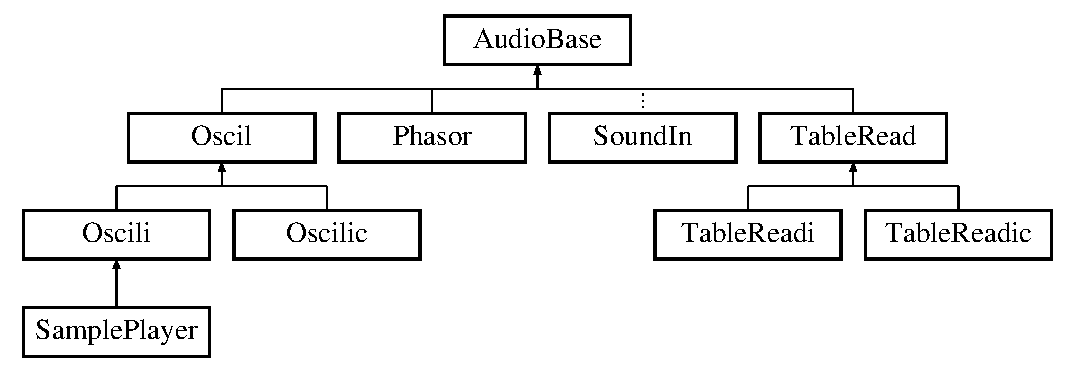
\includegraphics[height=4.000000cm]{class_audio_base}
\end{center}
\end{figure}
\subsection*{Public Member Functions}
\begin{DoxyCompactItemize}
\item 
\hyperlink{class_audio_base_adc5c0107a42e484ac18ca6f3be49785c}{Audio\+Base} (uint32\+\_\+t nchnls=def\+\_\+nchnls, double sr=def\+\_\+sr, double vsize=def\+\_\+vsize)
\item 
virtual \hyperlink{class_audio_base_a6517030ff62530ae78c7fa63a9512c6d}{$\sim$\+Audio\+Base} ()
\item 
double $\ast$ \hyperlink{class_audio_base_adcdfe60eebbc745101dd0437874ec237}{output} ()
\item 
double \hyperlink{class_audio_base_a51df052f8e916fff79df78558c0193b4}{output} (uint32\+\_\+t ndx)
\end{DoxyCompactItemize}


\subsection{Detailed Description}
Audio D\+SP base class 

\subsection{Constructor \& Destructor Documentation}
\mbox{\Hypertarget{class_audio_base_adc5c0107a42e484ac18ca6f3be49785c}\label{class_audio_base_adc5c0107a42e484ac18ca6f3be49785c}} 
\index{Audio\+Base@{Audio\+Base}!Audio\+Base@{Audio\+Base}}
\index{Audio\+Base@{Audio\+Base}!Audio\+Base@{Audio\+Base}}
\subsubsection{\texorpdfstring{Audio\+Base()}{AudioBase()}}
{\footnotesize\ttfamily Audio\+Base\+::\+Audio\+Base (\begin{DoxyParamCaption}\item[{uint32\+\_\+t}]{nchnls = {\ttfamily def\+\_\+nchnls},  }\item[{double}]{sr = {\ttfamily def\+\_\+sr},  }\item[{double}]{vsize = {\ttfamily def\+\_\+vsize} }\end{DoxyParamCaption})\hspace{0.3cm}{\ttfamily [inline]}}

\hyperlink{class_audio_base}{Audio\+Base} constructor ~\newline
~\newline
nchnls -\/ number of channels ~\newline
sr -\/ sampling rate ~\newline
vsize -\/ vector size (frames) ~\newline
\mbox{\Hypertarget{class_audio_base_a6517030ff62530ae78c7fa63a9512c6d}\label{class_audio_base_a6517030ff62530ae78c7fa63a9512c6d}} 
\index{Audio\+Base@{Audio\+Base}!````~Audio\+Base@{$\sim$\+Audio\+Base}}
\index{````~Audio\+Base@{$\sim$\+Audio\+Base}!Audio\+Base@{Audio\+Base}}
\subsubsection{\texorpdfstring{$\sim$\+Audio\+Base()}{~AudioBase()}}
{\footnotesize\ttfamily virtual Audio\+Base\+::$\sim$\+Audio\+Base (\begin{DoxyParamCaption}{ }\end{DoxyParamCaption})\hspace{0.3cm}{\ttfamily [inline]}, {\ttfamily [virtual]}}

\hyperlink{class_audio_base}{Audio\+Base} destructor 

\subsection{Member Function Documentation}
\mbox{\Hypertarget{class_audio_base_adcdfe60eebbc745101dd0437874ec237}\label{class_audio_base_adcdfe60eebbc745101dd0437874ec237}} 
\index{Audio\+Base@{Audio\+Base}!output@{output}}
\index{output@{output}!Audio\+Base@{Audio\+Base}}
\subsubsection{\texorpdfstring{output()}{output()}\hspace{0.1cm}{\footnotesize\ttfamily [1/2]}}
{\footnotesize\ttfamily double$\ast$ Audio\+Base\+::output (\begin{DoxyParamCaption}{ }\end{DoxyParamCaption})\hspace{0.3cm}{\ttfamily [inline]}}

Get the audio output vector \mbox{\Hypertarget{class_audio_base_a51df052f8e916fff79df78558c0193b4}\label{class_audio_base_a51df052f8e916fff79df78558c0193b4}} 
\index{Audio\+Base@{Audio\+Base}!output@{output}}
\index{output@{output}!Audio\+Base@{Audio\+Base}}
\subsubsection{\texorpdfstring{output()}{output()}\hspace{0.1cm}{\footnotesize\ttfamily [2/2]}}
{\footnotesize\ttfamily double Audio\+Base\+::output (\begin{DoxyParamCaption}\item[{uint32\+\_\+t}]{ndx }\end{DoxyParamCaption})\hspace{0.3cm}{\ttfamily [inline]}}

Get a single sample at ndx off the output audio vector 

The documentation for this class was generated from the following file\+:\begin{DoxyCompactItemize}
\item 
src/Audio\+Base.\+h\end{DoxyCompactItemize}

\hypertarget{class_fourier_table}{}\section{Fourier\+Table Class Reference}
\label{class_fourier_table}\index{Fourier\+Table@{Fourier\+Table}}


{\ttfamily \#include $<$Fourier\+Table.\+h$>$}

Inheritance diagram for Fourier\+Table\+:\begin{figure}[H]
\begin{center}
\leavevmode
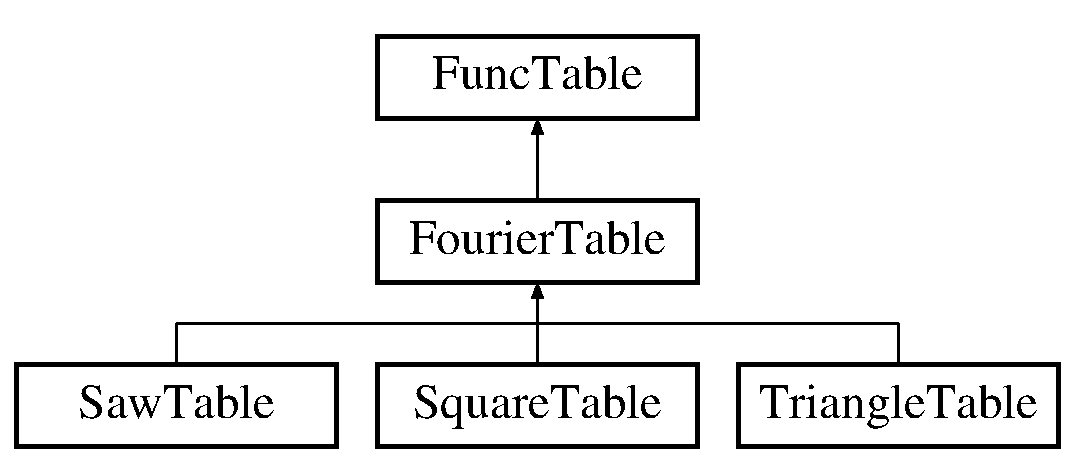
\includegraphics[height=3.000000cm]{class_fourier_table}
\end{center}
\end{figure}
\subsection*{Public Member Functions}
\begin{DoxyCompactItemize}
\item 
\hyperlink{class_fourier_table_ae208f9476736fdc0fe915773374d6e5b}{Fourier\+Table} (uint32\+\_\+t harms, double $\ast$amps=N\+U\+LL, double phase=0., uint32\+\_\+t tsize=def\+\_\+tsize)
\item 
\hyperlink{class_fourier_table_ac45625fd3a53952e75131fb8ea029432}{Fourier\+Table} (uint32\+\_\+t harms, uint32\+\_\+t type=S\+A\+W\+\_\+\+T\+A\+B\+LE, uint32\+\_\+t tsize=def\+\_\+tsize)
\end{DoxyCompactItemize}
\subsection*{Protected Member Functions}
\begin{DoxyCompactItemize}
\item 
void \hyperlink{class_fourier_table_af1c940238cc8e2c9bdd7f77c3ada9867}{create} (uint32\+\_\+t harms, double $\ast$amps, double phase)
\end{DoxyCompactItemize}


\subsection{Detailed Description}
Function tables based on Fourier Series 

\subsection{Constructor \& Destructor Documentation}
\mbox{\Hypertarget{class_fourier_table_ae208f9476736fdc0fe915773374d6e5b}\label{class_fourier_table_ae208f9476736fdc0fe915773374d6e5b}} 
\index{Fourier\+Table@{Fourier\+Table}!Fourier\+Table@{Fourier\+Table}}
\index{Fourier\+Table@{Fourier\+Table}!Fourier\+Table@{Fourier\+Table}}
\subsubsection{\texorpdfstring{Fourier\+Table()}{FourierTable()}\hspace{0.1cm}{\footnotesize\ttfamily [1/2]}}
{\footnotesize\ttfamily Fourier\+Table\+::\+Fourier\+Table (\begin{DoxyParamCaption}\item[{uint32\+\_\+t}]{harms,  }\item[{double $\ast$}]{amps = {\ttfamily NULL},  }\item[{double}]{phase = {\ttfamily 0.},  }\item[{uint32\+\_\+t}]{tsize = {\ttfamily def\+\_\+tsize} }\end{DoxyParamCaption})}

\hyperlink{class_fourier_table}{Fourier\+Table} constructor ~\newline
~\newline
harms -\/ number of harmonics ~\newline
amps -\/ array of harmonic amplitudes ~\newline
phase -\/ phase offset ~\newline
tsize -\/ table size ~\newline
\mbox{\Hypertarget{class_fourier_table_ac45625fd3a53952e75131fb8ea029432}\label{class_fourier_table_ac45625fd3a53952e75131fb8ea029432}} 
\index{Fourier\+Table@{Fourier\+Table}!Fourier\+Table@{Fourier\+Table}}
\index{Fourier\+Table@{Fourier\+Table}!Fourier\+Table@{Fourier\+Table}}
\subsubsection{\texorpdfstring{Fourier\+Table()}{FourierTable()}\hspace{0.1cm}{\footnotesize\ttfamily [2/2]}}
{\footnotesize\ttfamily Fourier\+Table\+::\+Fourier\+Table (\begin{DoxyParamCaption}\item[{uint32\+\_\+t}]{harms,  }\item[{uint32\+\_\+t}]{type = {\ttfamily SAW\+\_\+TABLE},  }\item[{uint32\+\_\+t}]{tsize = {\ttfamily def\+\_\+tsize} }\end{DoxyParamCaption})}

\hyperlink{class_fourier_table}{Fourier\+Table} constructor ~\newline
~\newline
harms -\/ number of harmonics ~\newline
type -\/ wave type ~\newline
tsize -\/ table size ~\newline


\subsection{Member Function Documentation}
\mbox{\Hypertarget{class_fourier_table_af1c940238cc8e2c9bdd7f77c3ada9867}\label{class_fourier_table_af1c940238cc8e2c9bdd7f77c3ada9867}} 
\index{Fourier\+Table@{Fourier\+Table}!create@{create}}
\index{create@{create}!Fourier\+Table@{Fourier\+Table}}
\subsubsection{\texorpdfstring{create()}{create()}}
{\footnotesize\ttfamily void Fourier\+Table\+::create (\begin{DoxyParamCaption}\item[{uint32\+\_\+t}]{harms,  }\item[{double $\ast$}]{amps,  }\item[{double}]{phase }\end{DoxyParamCaption})\hspace{0.3cm}{\ttfamily [protected]}}

Create the table 

The documentation for this class was generated from the following files\+:\begin{DoxyCompactItemize}
\item 
src/Fourier\+Table.\+h\item 
src/Fourier\+Table.\+cpp\end{DoxyCompactItemize}

\hypertarget{class_func_table}{}\section{Func\+Table Class Reference}
\label{class_func_table}\index{Func\+Table@{Func\+Table}}


{\ttfamily \#include $<$Func\+Table.\+h$>$}

Inheritance diagram for Func\+Table\+:\begin{figure}[H]
\begin{center}
\leavevmode
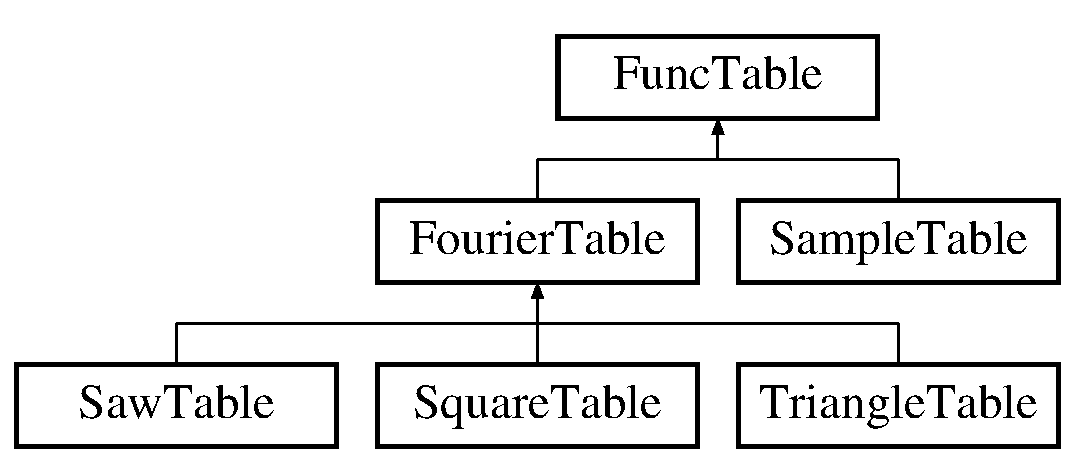
\includegraphics[height=3.000000cm]{class_func_table}
\end{center}
\end{figure}
\subsection*{Public Member Functions}
\begin{DoxyCompactItemize}
\item 
\hyperlink{class_func_table_ad76b1221806cebf553bfad4f8b39ac75}{Func\+Table} (uint32\+\_\+t tsize=def\+\_\+tsize)
\item 
double $\ast$ \hyperlink{class_func_table_aad16cb2dbc27ffe7b3b6ed3715657cc4}{table} ()
\item 
double \hyperlink{class_func_table_a6a7a98c7060fed37cf8a6d8823d7e33b}{table} (uint32\+\_\+t pos)
\end{DoxyCompactItemize}
\subsection*{Protected Member Functions}
\begin{DoxyCompactItemize}
\item 
void \hyperlink{class_func_table_af09474fb6b023d82597b940bf60ab71c}{normalise\+\_\+table} ()
\end{DoxyCompactItemize}


\subsection{Detailed Description}
Function table base class 

\subsection{Constructor \& Destructor Documentation}
\mbox{\Hypertarget{class_func_table_ad76b1221806cebf553bfad4f8b39ac75}\label{class_func_table_ad76b1221806cebf553bfad4f8b39ac75}} 
\index{Func\+Table@{Func\+Table}!Func\+Table@{Func\+Table}}
\index{Func\+Table@{Func\+Table}!Func\+Table@{Func\+Table}}
\subsubsection{\texorpdfstring{Func\+Table()}{FuncTable()}}
{\footnotesize\ttfamily Func\+Table\+::\+Func\+Table (\begin{DoxyParamCaption}\item[{uint32\+\_\+t}]{tsize = {\ttfamily def\+\_\+tsize} }\end{DoxyParamCaption})\hspace{0.3cm}{\ttfamily [inline]}}

\hyperlink{class_func_table}{Func\+Table} constructor ~\newline
~\newline
tsize -\/ table size ~\newline


\subsection{Member Function Documentation}
\mbox{\Hypertarget{class_func_table_af09474fb6b023d82597b940bf60ab71c}\label{class_func_table_af09474fb6b023d82597b940bf60ab71c}} 
\index{Func\+Table@{Func\+Table}!normalise\+\_\+table@{normalise\+\_\+table}}
\index{normalise\+\_\+table@{normalise\+\_\+table}!Func\+Table@{Func\+Table}}
\subsubsection{\texorpdfstring{normalise\+\_\+table()}{normalise\_table()}}
{\footnotesize\ttfamily void Func\+Table\+::normalise\+\_\+table (\begin{DoxyParamCaption}{ }\end{DoxyParamCaption})\hspace{0.3cm}{\ttfamily [inline]}, {\ttfamily [protected]}}

Normalise the table \mbox{\Hypertarget{class_func_table_aad16cb2dbc27ffe7b3b6ed3715657cc4}\label{class_func_table_aad16cb2dbc27ffe7b3b6ed3715657cc4}} 
\index{Func\+Table@{Func\+Table}!table@{table}}
\index{table@{table}!Func\+Table@{Func\+Table}}
\subsubsection{\texorpdfstring{table()}{table()}\hspace{0.1cm}{\footnotesize\ttfamily [1/2]}}
{\footnotesize\ttfamily double$\ast$ Func\+Table\+::table (\begin{DoxyParamCaption}{ }\end{DoxyParamCaption})\hspace{0.3cm}{\ttfamily [inline]}}

Get the function table \mbox{\Hypertarget{class_func_table_a6a7a98c7060fed37cf8a6d8823d7e33b}\label{class_func_table_a6a7a98c7060fed37cf8a6d8823d7e33b}} 
\index{Func\+Table@{Func\+Table}!table@{table}}
\index{table@{table}!Func\+Table@{Func\+Table}}
\subsubsection{\texorpdfstring{table()}{table()}\hspace{0.1cm}{\footnotesize\ttfamily [2/2]}}
{\footnotesize\ttfamily double Func\+Table\+::table (\begin{DoxyParamCaption}\item[{uint32\+\_\+t}]{pos }\end{DoxyParamCaption})\hspace{0.3cm}{\ttfamily [inline]}}

Get a single point at pos from the function table 

The documentation for this class was generated from the following file\+:\begin{DoxyCompactItemize}
\item 
src/Func\+Table.\+h\end{DoxyCompactItemize}

\hypertarget{class_oscil}{}\section{Oscil Class Reference}
\label{class_oscil}\index{Oscil@{Oscil}}


{\ttfamily \#include $<$Oscil.\+h$>$}

Inheritance diagram for Oscil\+:\begin{figure}[H]
\begin{center}
\leavevmode
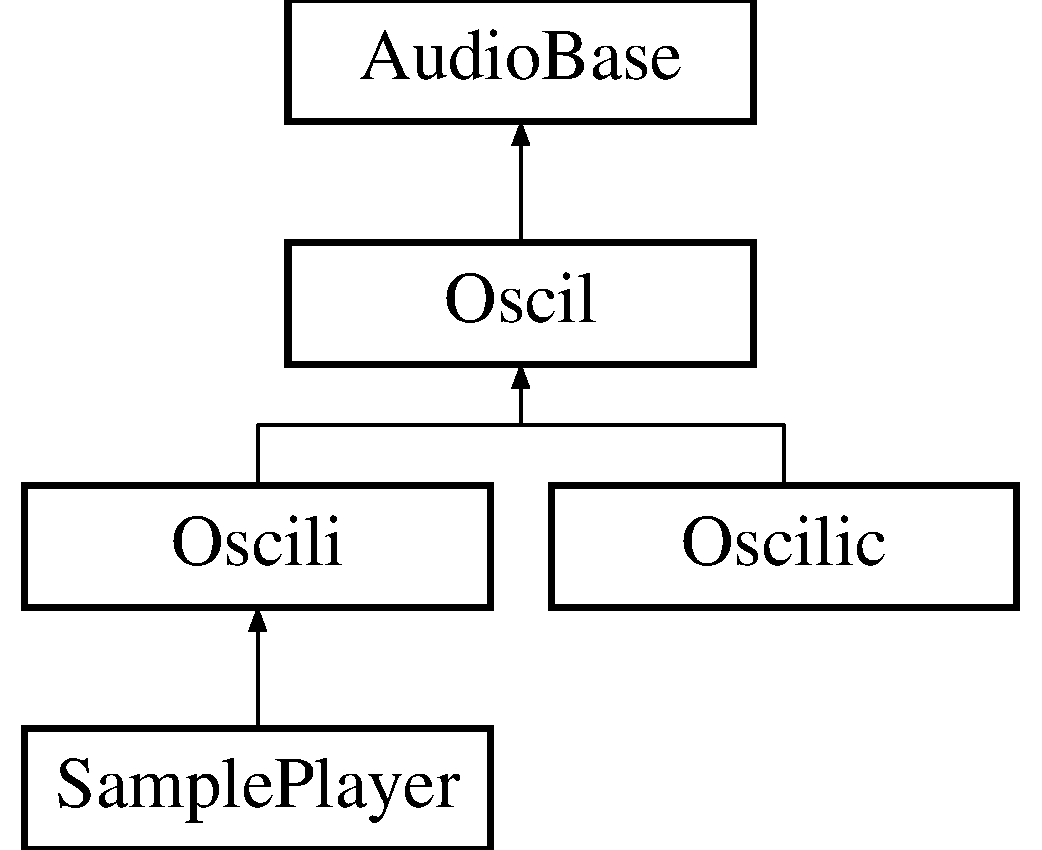
\includegraphics[height=4.000000cm]{class_oscil}
\end{center}
\end{figure}
\subsection*{Public Member Functions}
\begin{DoxyCompactItemize}
\item 
\hyperlink{class_oscil_a02ed65e22d9046e3f6253281b107b7bd}{Oscil} (double amp, double freq, double phase=.\+0, double $\ast$table=N\+U\+LL, uint32\+\_\+t tsize=def\+\_\+tsize, double sr=def\+\_\+sr, uint32\+\_\+t vsize=def\+\_\+vsize)
\item 
virtual \hyperlink{class_oscil_a3c09a41fb42bce840ca1b27cf27cf4f1}{$\sim$\+Oscil} ()
\item 
virtual void \hyperlink{class_oscil_a0e658a6f1b494286a783ce63e95f48ba}{process} ()
\item 
virtual void \hyperlink{class_oscil_a7ed04cfd228e849ddf95d09ea0aee8c2}{process} (double amp)
\item 
virtual void \hyperlink{class_oscil_abca4352d264fd66538502c72c2440784}{process} (double amp, double freq)
\end{DoxyCompactItemize}
\subsection*{Protected Member Functions}
\begin{DoxyCompactItemize}
\item 
void \hyperlink{class_oscil_a2dc5570e853d1364f753ff88f62d4e64}{mod} ()
\end{DoxyCompactItemize}


\subsection{Detailed Description}
Truncating oscillator 

\subsection{Constructor \& Destructor Documentation}
\mbox{\Hypertarget{class_oscil_a02ed65e22d9046e3f6253281b107b7bd}\label{class_oscil_a02ed65e22d9046e3f6253281b107b7bd}} 
\index{Oscil@{Oscil}!Oscil@{Oscil}}
\index{Oscil@{Oscil}!Oscil@{Oscil}}
\subsubsection{\texorpdfstring{Oscil()}{Oscil()}}
{\footnotesize\ttfamily Oscil\+::\+Oscil (\begin{DoxyParamCaption}\item[{double}]{amp,  }\item[{double}]{freq,  }\item[{double}]{phase = {\ttfamily .0},  }\item[{double $\ast$}]{table = {\ttfamily NULL},  }\item[{uint32\+\_\+t}]{tsize = {\ttfamily def\+\_\+tsize},  }\item[{double}]{sr = {\ttfamily def\+\_\+sr},  }\item[{uint32\+\_\+t}]{vsize = {\ttfamily def\+\_\+vsize} }\end{DoxyParamCaption})}

\hyperlink{class_oscil}{Oscil} constructor ~\newline
~\newline
amp -\/ amplitude ~\newline
freq -\/ frequency in Hz ~\newline
phase -\/ init phase (0-\/1) ~\newline
 table -\/ function table ~\newline
tsize -\/ table size ~\newline
sr -\/ sampling rate ~\newline
vsize -\/ vector size ~\newline
\mbox{\Hypertarget{class_oscil_a3c09a41fb42bce840ca1b27cf27cf4f1}\label{class_oscil_a3c09a41fb42bce840ca1b27cf27cf4f1}} 
\index{Oscil@{Oscil}!````~Oscil@{$\sim$\+Oscil}}
\index{````~Oscil@{$\sim$\+Oscil}!Oscil@{Oscil}}
\subsubsection{\texorpdfstring{$\sim$\+Oscil()}{~Oscil()}}
{\footnotesize\ttfamily Oscil\+::$\sim$\+Oscil (\begin{DoxyParamCaption}{ }\end{DoxyParamCaption})\hspace{0.3cm}{\ttfamily [virtual]}}

\hyperlink{class_oscil}{Oscil} destructor 

\subsection{Member Function Documentation}
\mbox{\Hypertarget{class_oscil_a2dc5570e853d1364f753ff88f62d4e64}\label{class_oscil_a2dc5570e853d1364f753ff88f62d4e64}} 
\index{Oscil@{Oscil}!mod@{mod}}
\index{mod@{mod}!Oscil@{Oscil}}
\subsubsection{\texorpdfstring{mod()}{mod()}}
{\footnotesize\ttfamily void Oscil\+::mod (\begin{DoxyParamCaption}{ }\end{DoxyParamCaption})\hspace{0.3cm}{\ttfamily [inline]}, {\ttfamily [protected]}}

phase modulo \mbox{\Hypertarget{class_oscil_a0e658a6f1b494286a783ce63e95f48ba}\label{class_oscil_a0e658a6f1b494286a783ce63e95f48ba}} 
\index{Oscil@{Oscil}!process@{process}}
\index{process@{process}!Oscil@{Oscil}}
\subsubsection{\texorpdfstring{process()}{process()}\hspace{0.1cm}{\footnotesize\ttfamily [1/3]}}
{\footnotesize\ttfamily void Oscil\+::process (\begin{DoxyParamCaption}{ }\end{DoxyParamCaption})\hspace{0.3cm}{\ttfamily [virtual]}}

Process one vector of audio 

Reimplemented in \hyperlink{class_oscilic_adcff5c6c3fd5a4da4bc76e05091d6dda}{Oscilic}, \hyperlink{class_sample_player_a263ee55c5d334486bc57956458a64713}{Sample\+Player}, and \hyperlink{class_oscili_a2571464f3b4874c3ca691061e8db7d32}{Oscili}.

\mbox{\Hypertarget{class_oscil_a7ed04cfd228e849ddf95d09ea0aee8c2}\label{class_oscil_a7ed04cfd228e849ddf95d09ea0aee8c2}} 
\index{Oscil@{Oscil}!process@{process}}
\index{process@{process}!Oscil@{Oscil}}
\subsubsection{\texorpdfstring{process()}{process()}\hspace{0.1cm}{\footnotesize\ttfamily [2/3]}}
{\footnotesize\ttfamily virtual void Oscil\+::process (\begin{DoxyParamCaption}\item[{double}]{amp }\end{DoxyParamCaption})\hspace{0.3cm}{\ttfamily [inline]}, {\ttfamily [virtual]}}

Process one vector of audio with amplitude amp 

Reimplemented in \hyperlink{class_sample_player_a806595c5e7674717d52bb8a57f451c0b}{Sample\+Player}, \hyperlink{class_oscilic_ad97eaf877abdd40fc06499198eb3d9bc}{Oscilic}, and \hyperlink{class_oscili_a1fb47dff09f771481e1a1d2fde39d775}{Oscili}.

\mbox{\Hypertarget{class_oscil_abca4352d264fd66538502c72c2440784}\label{class_oscil_abca4352d264fd66538502c72c2440784}} 
\index{Oscil@{Oscil}!process@{process}}
\index{process@{process}!Oscil@{Oscil}}
\subsubsection{\texorpdfstring{process()}{process()}\hspace{0.1cm}{\footnotesize\ttfamily [3/3]}}
{\footnotesize\ttfamily virtual void Oscil\+::process (\begin{DoxyParamCaption}\item[{double}]{amp,  }\item[{double}]{freq }\end{DoxyParamCaption})\hspace{0.3cm}{\ttfamily [inline]}, {\ttfamily [virtual]}}

Process one vector of audio with amplitude amp and frequency freq 

Reimplemented in \hyperlink{class_sample_player_a01fc7c2fdfd29c0c178e288d5aa06acc}{Sample\+Player}, \hyperlink{class_oscilic_acce96320f114bbd74114ef87e39660aa}{Oscilic}, and \hyperlink{class_oscili_a053ace3b633b645c4b8a517009ea7389}{Oscili}.



The documentation for this class was generated from the following files\+:\begin{DoxyCompactItemize}
\item 
src/Oscil.\+h\item 
src/Oscil.\+cpp\end{DoxyCompactItemize}

\hypertarget{class_oscili}{}\section{Oscili Class Reference}
\label{class_oscili}\index{Oscili@{Oscili}}


{\ttfamily \#include $<$Oscili.\+h$>$}

Inheritance diagram for Oscili\+:\begin{figure}[H]
\begin{center}
\leavevmode
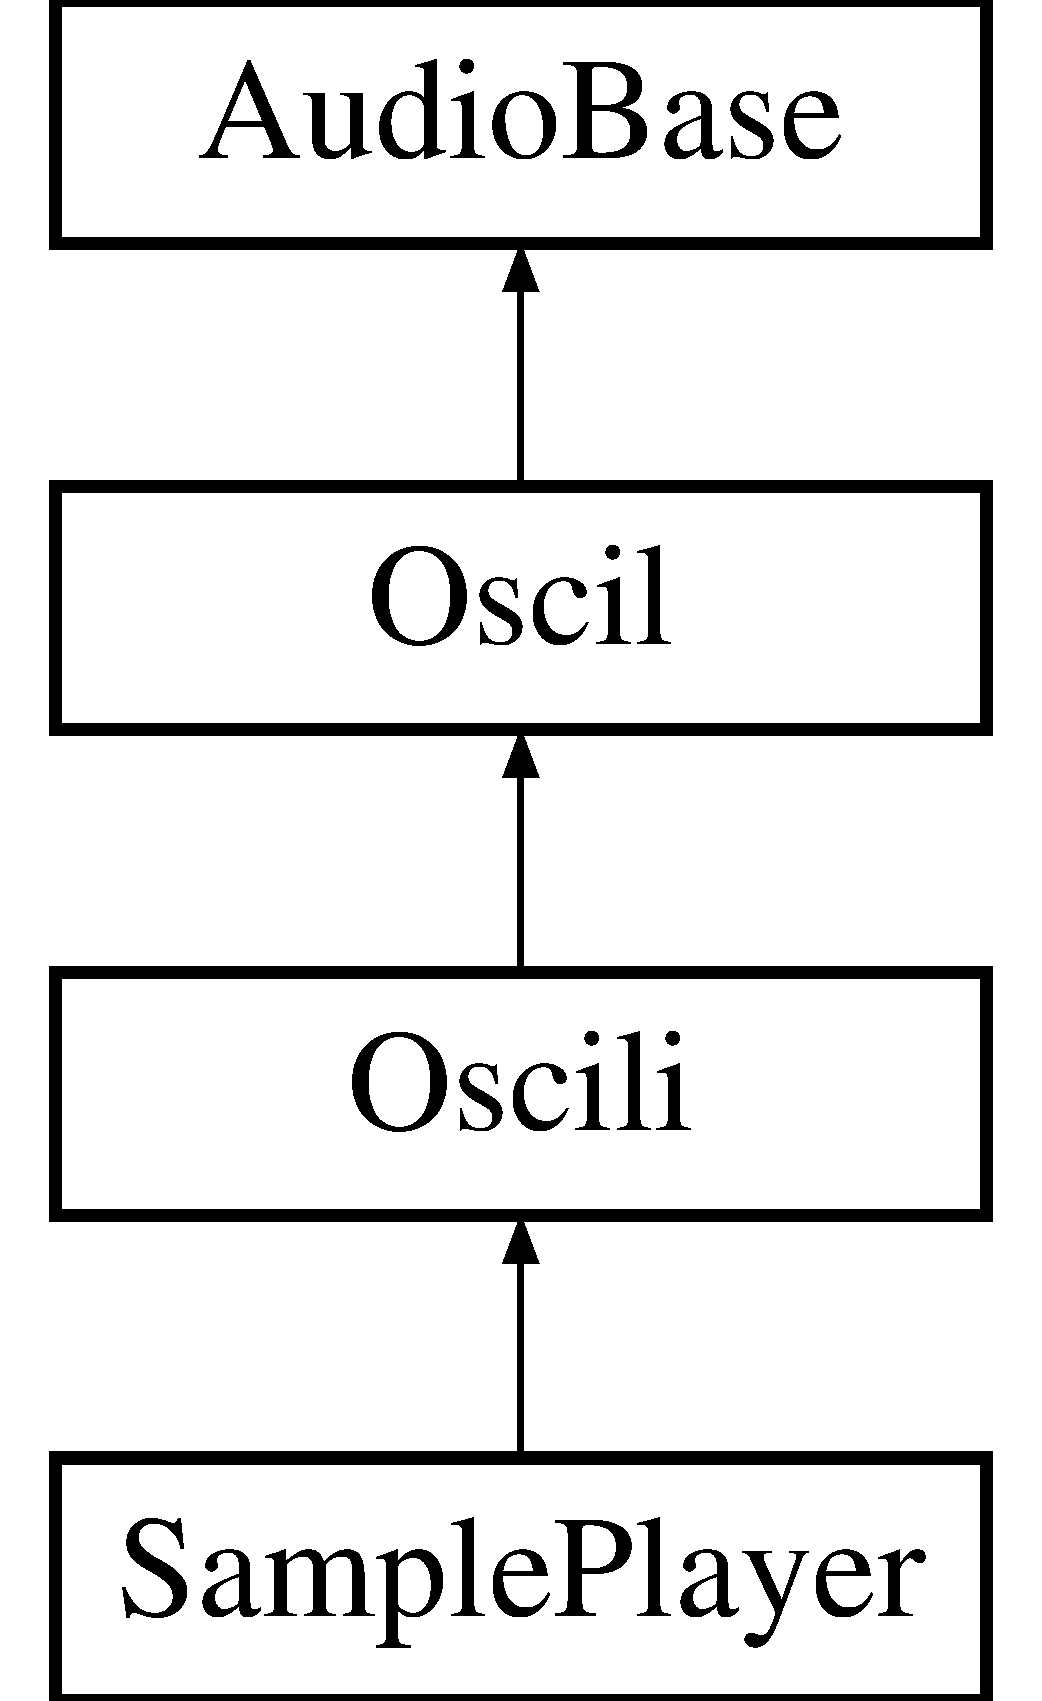
\includegraphics[height=4.000000cm]{class_oscili}
\end{center}
\end{figure}
\subsection*{Public Member Functions}
\begin{DoxyCompactItemize}
\item 
\hyperlink{class_oscili_a67e6c220007c24a72456680645c0bfa0}{Oscili} (double amp, double freq, double phase=.\+0, double $\ast$table=N\+U\+LL, uint32\+\_\+t tsize=def\+\_\+tsize, double sr=def\+\_\+sr, uint32\+\_\+t vsize=def\+\_\+vsize)
\item 
virtual void \hyperlink{class_oscili_a2571464f3b4874c3ca691061e8db7d32}{process} ()
\item 
virtual void \hyperlink{class_oscili_a1fb47dff09f771481e1a1d2fde39d775}{process} (double amp)
\item 
virtual void \hyperlink{class_oscili_a053ace3b633b645c4b8a517009ea7389}{process} (double amp, double freq)
\end{DoxyCompactItemize}
\subsection*{Additional Inherited Members}


\subsection{Detailed Description}
Linear interpolation oscillator 

\subsection{Constructor \& Destructor Documentation}
\mbox{\Hypertarget{class_oscili_a67e6c220007c24a72456680645c0bfa0}\label{class_oscili_a67e6c220007c24a72456680645c0bfa0}} 
\index{Oscili@{Oscili}!Oscili@{Oscili}}
\index{Oscili@{Oscili}!Oscili@{Oscili}}
\subsubsection{\texorpdfstring{Oscili()}{Oscili()}}
{\footnotesize\ttfamily Oscili\+::\+Oscili (\begin{DoxyParamCaption}\item[{double}]{amp,  }\item[{double}]{freq,  }\item[{double}]{phase = {\ttfamily .0},  }\item[{double $\ast$}]{table = {\ttfamily NULL},  }\item[{uint32\+\_\+t}]{tsize = {\ttfamily def\+\_\+tsize},  }\item[{double}]{sr = {\ttfamily def\+\_\+sr},  }\item[{uint32\+\_\+t}]{vsize = {\ttfamily def\+\_\+vsize} }\end{DoxyParamCaption})\hspace{0.3cm}{\ttfamily [inline]}}

\hyperlink{class_oscili}{Oscili} constructor ~\newline
~\newline
amp -\/ amplitude ~\newline
freq -\/ frequency in Hz ~\newline
phase -\/ init phase (0-\/1) ~\newline
 table -\/ function table ~\newline
tsize -\/ table size ~\newline
sr -\/ sampling rate ~\newline
vsize -\/ vector size ~\newline


\subsection{Member Function Documentation}
\mbox{\Hypertarget{class_oscili_a2571464f3b4874c3ca691061e8db7d32}\label{class_oscili_a2571464f3b4874c3ca691061e8db7d32}} 
\index{Oscili@{Oscili}!process@{process}}
\index{process@{process}!Oscili@{Oscili}}
\subsubsection{\texorpdfstring{process()}{process()}\hspace{0.1cm}{\footnotesize\ttfamily [1/3]}}
{\footnotesize\ttfamily void Oscili\+::process (\begin{DoxyParamCaption}{ }\end{DoxyParamCaption})\hspace{0.3cm}{\ttfamily [virtual]}}

Process one vector of audio 

Reimplemented from \hyperlink{class_oscil_a0e658a6f1b494286a783ce63e95f48ba}{Oscil}.



Reimplemented in \hyperlink{class_sample_player_a263ee55c5d334486bc57956458a64713}{Sample\+Player}.

\mbox{\Hypertarget{class_oscili_a1fb47dff09f771481e1a1d2fde39d775}\label{class_oscili_a1fb47dff09f771481e1a1d2fde39d775}} 
\index{Oscili@{Oscili}!process@{process}}
\index{process@{process}!Oscili@{Oscili}}
\subsubsection{\texorpdfstring{process()}{process()}\hspace{0.1cm}{\footnotesize\ttfamily [2/3]}}
{\footnotesize\ttfamily virtual void Oscili\+::process (\begin{DoxyParamCaption}\item[{double}]{amp }\end{DoxyParamCaption})\hspace{0.3cm}{\ttfamily [inline]}, {\ttfamily [virtual]}}

Process one vector of audio with amplitude amp 

Reimplemented from \hyperlink{class_oscil_a7ed04cfd228e849ddf95d09ea0aee8c2}{Oscil}.



Reimplemented in \hyperlink{class_sample_player_a806595c5e7674717d52bb8a57f451c0b}{Sample\+Player}.

\mbox{\Hypertarget{class_oscili_a053ace3b633b645c4b8a517009ea7389}\label{class_oscili_a053ace3b633b645c4b8a517009ea7389}} 
\index{Oscili@{Oscili}!process@{process}}
\index{process@{process}!Oscili@{Oscili}}
\subsubsection{\texorpdfstring{process()}{process()}\hspace{0.1cm}{\footnotesize\ttfamily [3/3]}}
{\footnotesize\ttfamily virtual void Oscili\+::process (\begin{DoxyParamCaption}\item[{double}]{amp,  }\item[{double}]{freq }\end{DoxyParamCaption})\hspace{0.3cm}{\ttfamily [inline]}, {\ttfamily [virtual]}}

Process one vector of audio with amplitude amp and frequency freq 

Reimplemented from \hyperlink{class_oscil_abca4352d264fd66538502c72c2440784}{Oscil}.



Reimplemented in \hyperlink{class_sample_player_a01fc7c2fdfd29c0c178e288d5aa06acc}{Sample\+Player}.



The documentation for this class was generated from the following files\+:\begin{DoxyCompactItemize}
\item 
src/Oscili.\+h\item 
src/Oscili.\+cpp\end{DoxyCompactItemize}

\hypertarget{class_oscilic}{}\section{Oscilic Class Reference}
\label{class_oscilic}\index{Oscilic@{Oscilic}}


{\ttfamily \#include $<$Oscilic.\+h$>$}

Inheritance diagram for Oscilic\+:\begin{figure}[H]
\begin{center}
\leavevmode
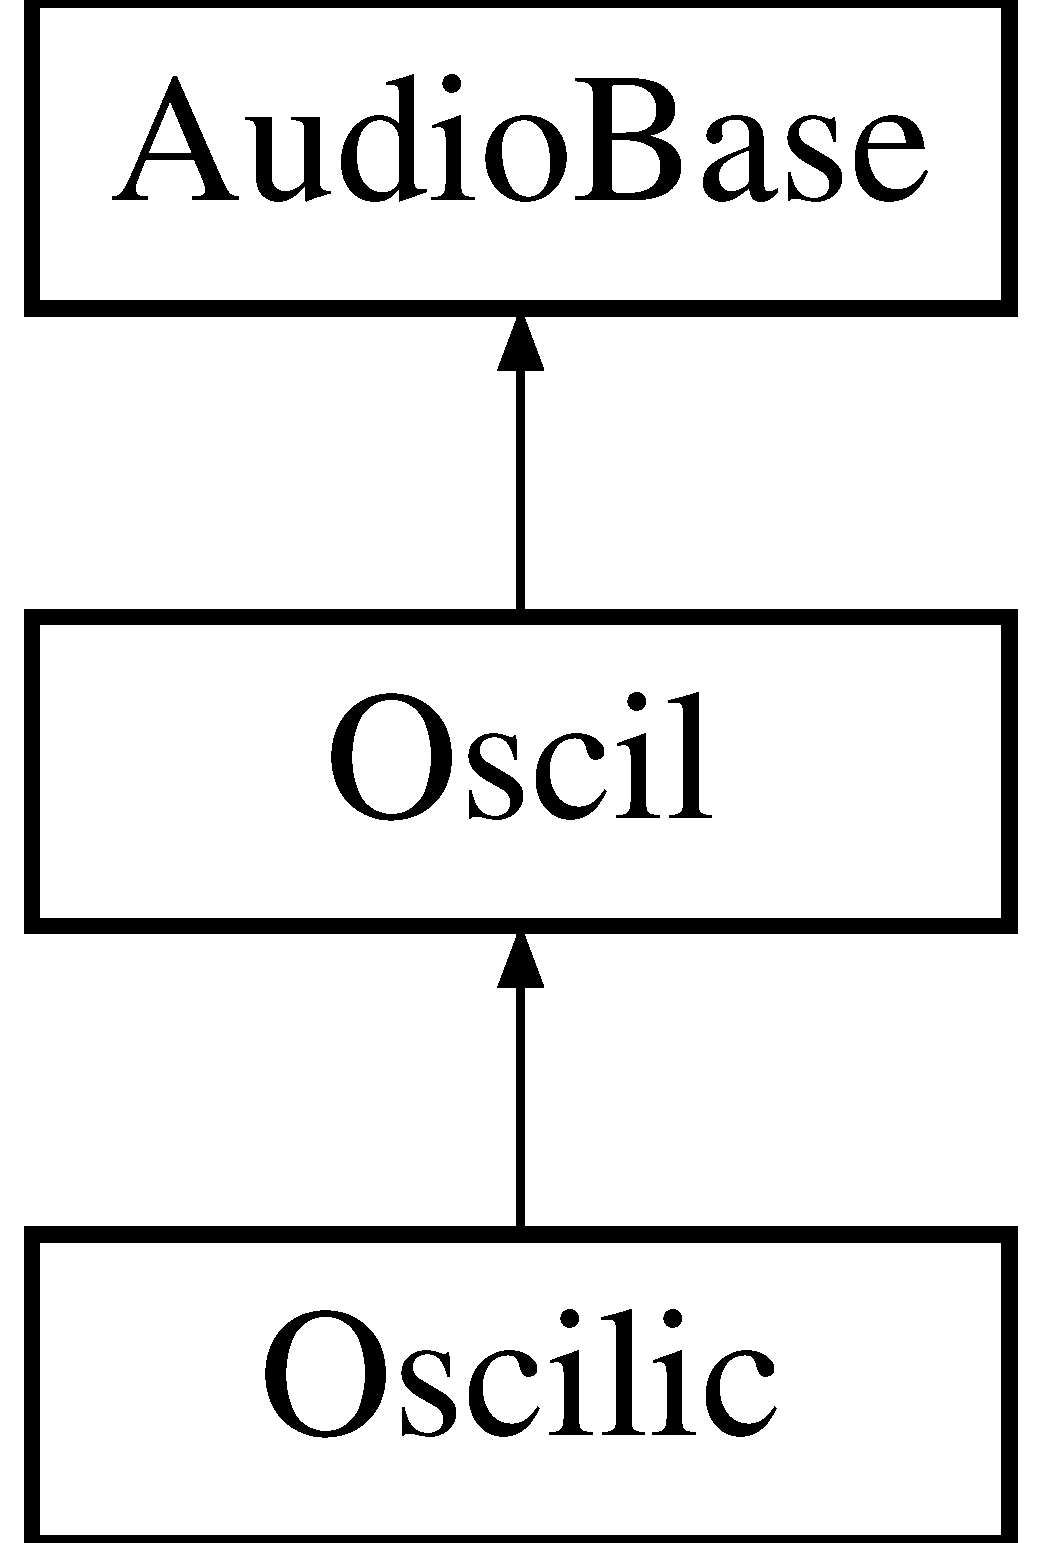
\includegraphics[height=3.000000cm]{class_oscilic}
\end{center}
\end{figure}
\subsection*{Public Member Functions}
\begin{DoxyCompactItemize}
\item 
\hyperlink{class_oscilic_a7518bfbb2bae80e100af56f5caf58cd8}{Oscilic} (double amp, double freq, double phase=.\+0, double $\ast$table=N\+U\+LL, uint32\+\_\+t tsize=def\+\_\+tsize, double sr=def\+\_\+sr, uint32\+\_\+t vsize=def\+\_\+vsize)
\item 
virtual void \hyperlink{class_oscilic_adcff5c6c3fd5a4da4bc76e05091d6dda}{process} ()
\item 
virtual void \hyperlink{class_oscilic_ad97eaf877abdd40fc06499198eb3d9bc}{process} (double amp)
\item 
virtual void \hyperlink{class_oscilic_acce96320f114bbd74114ef87e39660aa}{process} (double amp, double freq)
\end{DoxyCompactItemize}
\subsection*{Additional Inherited Members}


\subsection{Detailed Description}
Cubic interpolation oscillator 

\subsection{Constructor \& Destructor Documentation}
\mbox{\Hypertarget{class_oscilic_a7518bfbb2bae80e100af56f5caf58cd8}\label{class_oscilic_a7518bfbb2bae80e100af56f5caf58cd8}} 
\index{Oscilic@{Oscilic}!Oscilic@{Oscilic}}
\index{Oscilic@{Oscilic}!Oscilic@{Oscilic}}
\subsubsection{\texorpdfstring{Oscilic()}{Oscilic()}}
{\footnotesize\ttfamily Oscilic\+::\+Oscilic (\begin{DoxyParamCaption}\item[{double}]{amp,  }\item[{double}]{freq,  }\item[{double}]{phase = {\ttfamily .0},  }\item[{double $\ast$}]{table = {\ttfamily NULL},  }\item[{uint32\+\_\+t}]{tsize = {\ttfamily def\+\_\+tsize},  }\item[{double}]{sr = {\ttfamily def\+\_\+sr},  }\item[{uint32\+\_\+t}]{vsize = {\ttfamily def\+\_\+vsize} }\end{DoxyParamCaption})\hspace{0.3cm}{\ttfamily [inline]}}

\hyperlink{class_oscilic}{Oscilic} constructor ~\newline
~\newline
amp -\/ amplitude ~\newline
freq -\/ frequency in Hz ~\newline
phase -\/ init phase (0-\/1) ~\newline
 table -\/ function table ~\newline
tsize -\/ table size ~\newline
sr -\/ sampling rate ~\newline
vsize -\/ vector size ~\newline


\subsection{Member Function Documentation}
\mbox{\Hypertarget{class_oscilic_adcff5c6c3fd5a4da4bc76e05091d6dda}\label{class_oscilic_adcff5c6c3fd5a4da4bc76e05091d6dda}} 
\index{Oscilic@{Oscilic}!process@{process}}
\index{process@{process}!Oscilic@{Oscilic}}
\subsubsection{\texorpdfstring{process()}{process()}\hspace{0.1cm}{\footnotesize\ttfamily [1/3]}}
{\footnotesize\ttfamily void Oscilic\+::process (\begin{DoxyParamCaption}{ }\end{DoxyParamCaption})\hspace{0.3cm}{\ttfamily [virtual]}}

Process one vector of audio 

Reimplemented from \hyperlink{class_oscil_a0e658a6f1b494286a783ce63e95f48ba}{Oscil}.

\mbox{\Hypertarget{class_oscilic_ad97eaf877abdd40fc06499198eb3d9bc}\label{class_oscilic_ad97eaf877abdd40fc06499198eb3d9bc}} 
\index{Oscilic@{Oscilic}!process@{process}}
\index{process@{process}!Oscilic@{Oscilic}}
\subsubsection{\texorpdfstring{process()}{process()}\hspace{0.1cm}{\footnotesize\ttfamily [2/3]}}
{\footnotesize\ttfamily virtual void Oscilic\+::process (\begin{DoxyParamCaption}\item[{double}]{amp }\end{DoxyParamCaption})\hspace{0.3cm}{\ttfamily [inline]}, {\ttfamily [virtual]}}

Process one vector of audio with amplitude amp 

Reimplemented from \hyperlink{class_oscil_a7ed04cfd228e849ddf95d09ea0aee8c2}{Oscil}.

\mbox{\Hypertarget{class_oscilic_acce96320f114bbd74114ef87e39660aa}\label{class_oscilic_acce96320f114bbd74114ef87e39660aa}} 
\index{Oscilic@{Oscilic}!process@{process}}
\index{process@{process}!Oscilic@{Oscilic}}
\subsubsection{\texorpdfstring{process()}{process()}\hspace{0.1cm}{\footnotesize\ttfamily [3/3]}}
{\footnotesize\ttfamily virtual void Oscilic\+::process (\begin{DoxyParamCaption}\item[{double}]{amp,  }\item[{double}]{freq }\end{DoxyParamCaption})\hspace{0.3cm}{\ttfamily [inline]}, {\ttfamily [virtual]}}

Process one vector of audio with amplitude amp and frequency freq 

Reimplemented from \hyperlink{class_oscil_abca4352d264fd66538502c72c2440784}{Oscil}.



The documentation for this class was generated from the following files\+:\begin{DoxyCompactItemize}
\item 
src/Oscilic.\+h\item 
src/Oscilic.\+cpp\end{DoxyCompactItemize}

\hypertarget{class_phasor}{}\section{Phasor Class Reference}
\label{class_phasor}\index{Phasor@{Phasor}}


{\ttfamily \#include $<$Phasor.\+h$>$}

Inheritance diagram for Phasor\+:\begin{figure}[H]
\begin{center}
\leavevmode
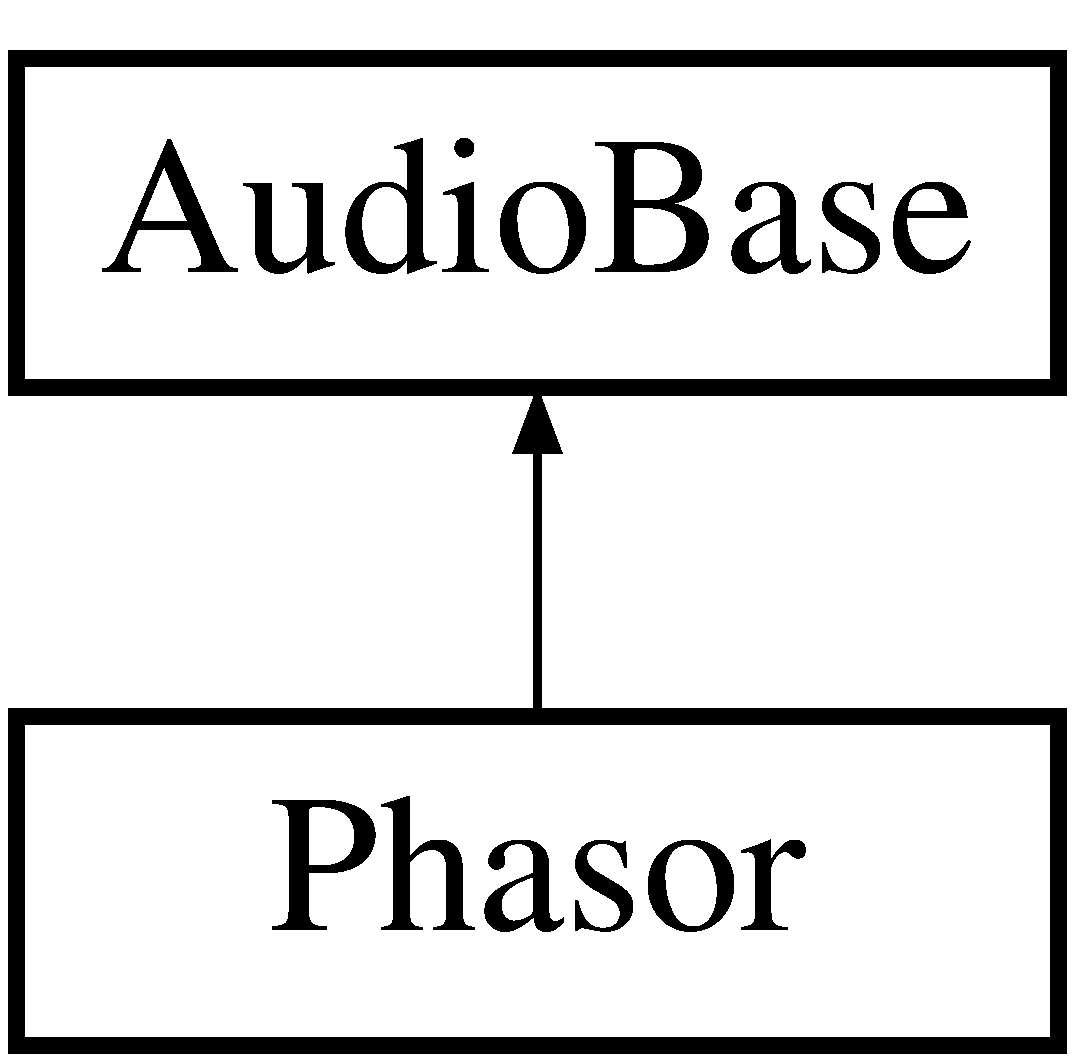
\includegraphics[height=2.000000cm]{class_phasor}
\end{center}
\end{figure}
\subsection*{Public Member Functions}
\begin{DoxyCompactItemize}
\item 
\hyperlink{class_phasor_a4522af2664d1a277de86e7a9eb053189}{Phasor} (double freq, double phase=.\+0, double sr=def\+\_\+sr, uint32\+\_\+t vsize=def\+\_\+vsize)
\item 
virtual void \hyperlink{class_phasor_abb4f4c04b5ca206ea79b8f9437bb1c33}{process} ()
\item 
virtual void \hyperlink{class_phasor_aa6a31e512e0f60497cc86de4467c33ef}{process} (double freq)
\end{DoxyCompactItemize}
\subsection*{Protected Member Functions}
\begin{DoxyCompactItemize}
\item 
void \hyperlink{class_phasor_a2a8267de2401d912bdd8fc25f2a38eb9}{mod} ()
\end{DoxyCompactItemize}


\subsection{Detailed Description}
Phase signal (ramp) generator 

\subsection{Constructor \& Destructor Documentation}
\mbox{\Hypertarget{class_phasor_a4522af2664d1a277de86e7a9eb053189}\label{class_phasor_a4522af2664d1a277de86e7a9eb053189}} 
\index{Phasor@{Phasor}!Phasor@{Phasor}}
\index{Phasor@{Phasor}!Phasor@{Phasor}}
\subsubsection{\texorpdfstring{Phasor()}{Phasor()}}
{\footnotesize\ttfamily Phasor\+::\+Phasor (\begin{DoxyParamCaption}\item[{double}]{freq,  }\item[{double}]{phase = {\ttfamily .0},  }\item[{double}]{sr = {\ttfamily def\+\_\+sr},  }\item[{uint32\+\_\+t}]{vsize = {\ttfamily def\+\_\+vsize} }\end{DoxyParamCaption})}

\hyperlink{class_phasor}{Phasor} constructor ~\newline
~\newline
freq -\/ frequency in Hz ~\newline
phase -\/ init phase (0-\/1) ~\newline
 sr -\/ sampling rate ~\newline
vsize -\/ vector size ~\newline


\subsection{Member Function Documentation}
\mbox{\Hypertarget{class_phasor_a2a8267de2401d912bdd8fc25f2a38eb9}\label{class_phasor_a2a8267de2401d912bdd8fc25f2a38eb9}} 
\index{Phasor@{Phasor}!mod@{mod}}
\index{mod@{mod}!Phasor@{Phasor}}
\subsubsection{\texorpdfstring{mod()}{mod()}}
{\footnotesize\ttfamily void Phasor\+::mod (\begin{DoxyParamCaption}{ }\end{DoxyParamCaption})\hspace{0.3cm}{\ttfamily [inline]}, {\ttfamily [protected]}}

phase modulo \mbox{\Hypertarget{class_phasor_abb4f4c04b5ca206ea79b8f9437bb1c33}\label{class_phasor_abb4f4c04b5ca206ea79b8f9437bb1c33}} 
\index{Phasor@{Phasor}!process@{process}}
\index{process@{process}!Phasor@{Phasor}}
\subsubsection{\texorpdfstring{process()}{process()}\hspace{0.1cm}{\footnotesize\ttfamily [1/2]}}
{\footnotesize\ttfamily void Phasor\+::process (\begin{DoxyParamCaption}{ }\end{DoxyParamCaption})\hspace{0.3cm}{\ttfamily [virtual]}}

Process one vector of audio \mbox{\Hypertarget{class_phasor_aa6a31e512e0f60497cc86de4467c33ef}\label{class_phasor_aa6a31e512e0f60497cc86de4467c33ef}} 
\index{Phasor@{Phasor}!process@{process}}
\index{process@{process}!Phasor@{Phasor}}
\subsubsection{\texorpdfstring{process()}{process()}\hspace{0.1cm}{\footnotesize\ttfamily [2/2]}}
{\footnotesize\ttfamily virtual void Phasor\+::process (\begin{DoxyParamCaption}\item[{double}]{freq }\end{DoxyParamCaption})\hspace{0.3cm}{\ttfamily [inline]}, {\ttfamily [virtual]}}

Process one vector of audio with frequency freq 

The documentation for this class was generated from the following files\+:\begin{DoxyCompactItemize}
\item 
src/Phasor.\+h\item 
src/Phasor.\+cpp\end{DoxyCompactItemize}

\hypertarget{class_sample_player}{}\section{Sample\+Player Class Reference}
\label{class_sample_player}\index{Sample\+Player@{Sample\+Player}}


{\ttfamily \#include $<$Sample\+Player.\+h$>$}

Inheritance diagram for Sample\+Player\+:\begin{figure}[H]
\begin{center}
\leavevmode
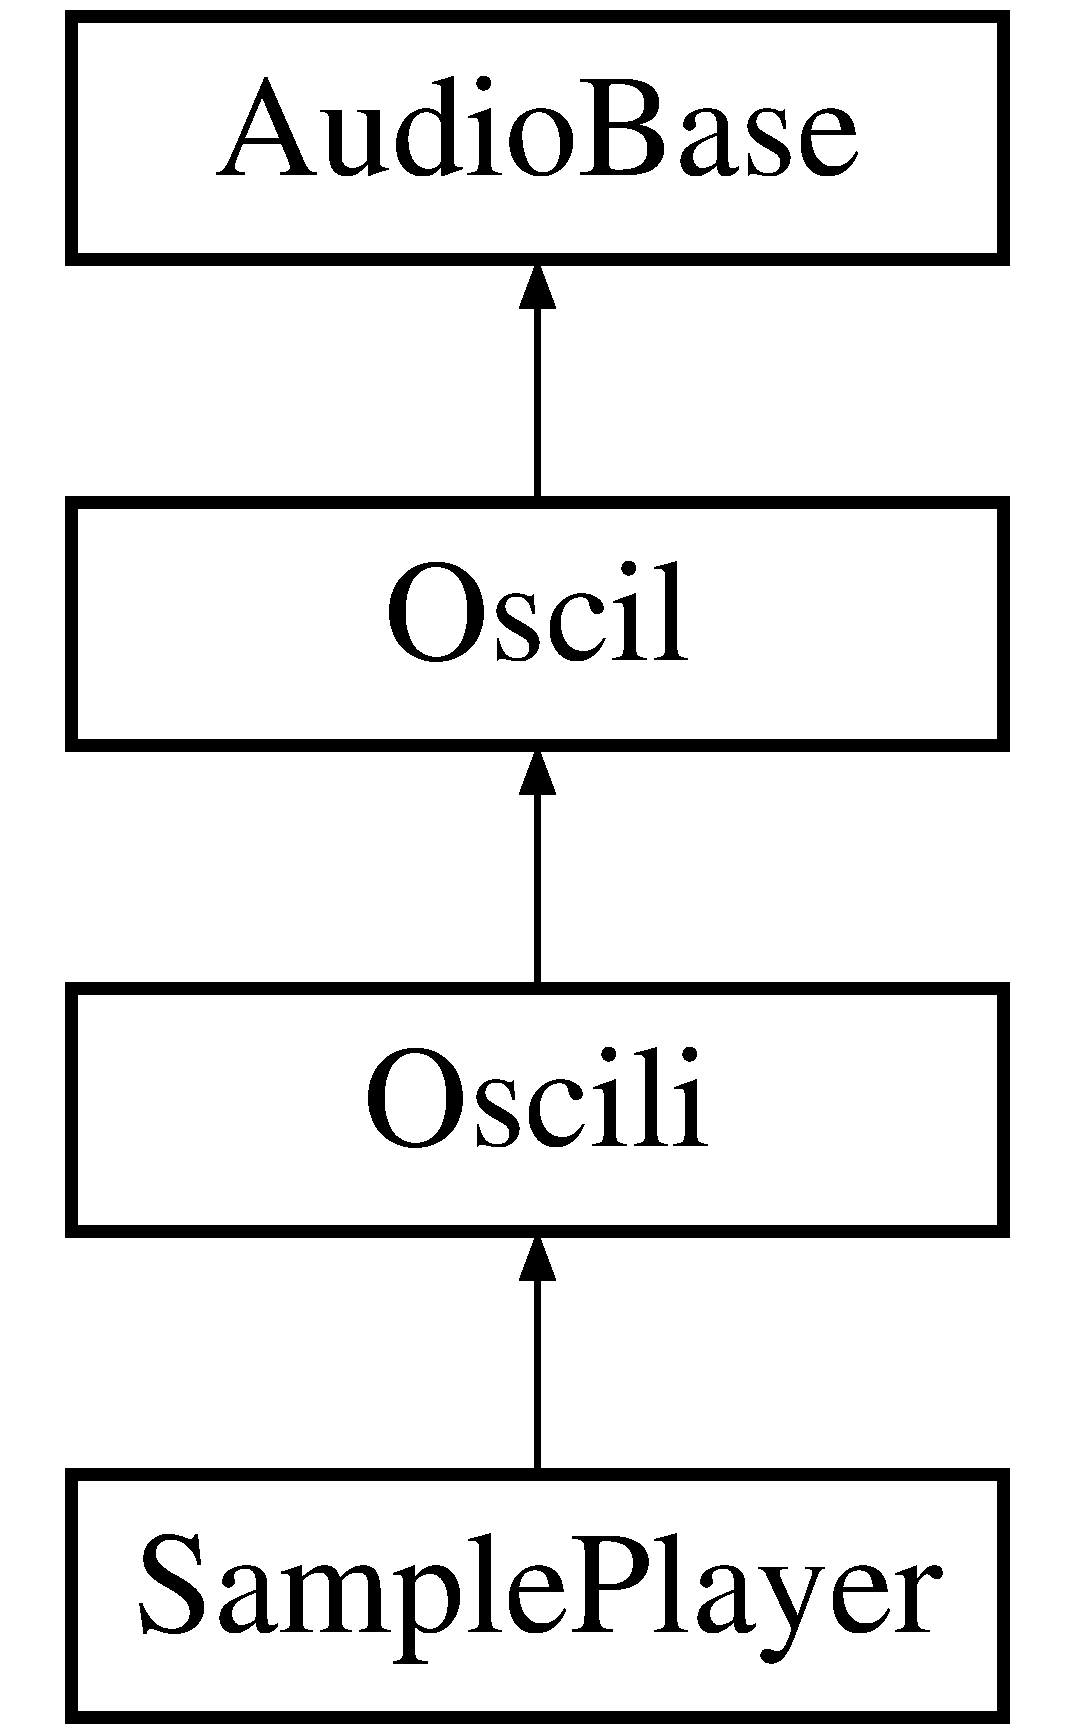
\includegraphics[height=4.000000cm]{class_sample_player}
\end{center}
\end{figure}
\subsection*{Public Member Functions}
\begin{DoxyCompactItemize}
\item 
\hyperlink{class_sample_player_aa7ce31700ed3ebebfb0604e642ca7ea8}{Sample\+Player} (double amp, double pitch, double phase=.\+0, double $\ast$table=N\+U\+LL, uint32\+\_\+t tsize=def\+\_\+tsize, double sr=def\+\_\+sr, uint32\+\_\+t vsize=def\+\_\+vsize)
\item 
virtual void \hyperlink{class_sample_player_a263ee55c5d334486bc57956458a64713}{process} ()
\item 
virtual void \hyperlink{class_sample_player_a806595c5e7674717d52bb8a57f451c0b}{process} (double amp)
\item 
virtual void \hyperlink{class_sample_player_a01fc7c2fdfd29c0c178e288d5aa06acc}{process} (double amp, double pitch)
\end{DoxyCompactItemize}
\subsection*{Additional Inherited Members}


\subsection{Detailed Description}
Sample playback oscillator with linear interpolation 

\subsection{Constructor \& Destructor Documentation}
\mbox{\Hypertarget{class_sample_player_aa7ce31700ed3ebebfb0604e642ca7ea8}\label{class_sample_player_aa7ce31700ed3ebebfb0604e642ca7ea8}} 
\index{Sample\+Player@{Sample\+Player}!Sample\+Player@{Sample\+Player}}
\index{Sample\+Player@{Sample\+Player}!Sample\+Player@{Sample\+Player}}
\subsubsection{\texorpdfstring{Sample\+Player()}{SamplePlayer()}}
{\footnotesize\ttfamily Sample\+Player\+::\+Sample\+Player (\begin{DoxyParamCaption}\item[{double}]{amp,  }\item[{double}]{pitch,  }\item[{double}]{phase = {\ttfamily .0},  }\item[{double $\ast$}]{table = {\ttfamily NULL},  }\item[{uint32\+\_\+t}]{tsize = {\ttfamily def\+\_\+tsize},  }\item[{double}]{sr = {\ttfamily def\+\_\+sr},  }\item[{uint32\+\_\+t}]{vsize = {\ttfamily def\+\_\+vsize} }\end{DoxyParamCaption})\hspace{0.3cm}{\ttfamily [inline]}}

\hyperlink{class_sample_player}{Sample\+Player} constructor ~\newline
~\newline
amp -\/ amplitude ~\newline
pitch -\/ playback pitch ~\newline
phase -\/ init phase (0-\/1) ~\newline
 table -\/ function table ~\newline
tsize -\/ table size ~\newline
sr -\/ sampling rate ~\newline
vsize -\/ vector size ~\newline


\subsection{Member Function Documentation}
\mbox{\Hypertarget{class_sample_player_a263ee55c5d334486bc57956458a64713}\label{class_sample_player_a263ee55c5d334486bc57956458a64713}} 
\index{Sample\+Player@{Sample\+Player}!process@{process}}
\index{process@{process}!Sample\+Player@{Sample\+Player}}
\subsubsection{\texorpdfstring{process()}{process()}\hspace{0.1cm}{\footnotesize\ttfamily [1/3]}}
{\footnotesize\ttfamily virtual void Sample\+Player\+::process (\begin{DoxyParamCaption}{ }\end{DoxyParamCaption})\hspace{0.3cm}{\ttfamily [inline]}, {\ttfamily [virtual]}}

Process one vector of audio 

Reimplemented from \hyperlink{class_oscili_a2571464f3b4874c3ca691061e8db7d32}{Oscili}.

\mbox{\Hypertarget{class_sample_player_a806595c5e7674717d52bb8a57f451c0b}\label{class_sample_player_a806595c5e7674717d52bb8a57f451c0b}} 
\index{Sample\+Player@{Sample\+Player}!process@{process}}
\index{process@{process}!Sample\+Player@{Sample\+Player}}
\subsubsection{\texorpdfstring{process()}{process()}\hspace{0.1cm}{\footnotesize\ttfamily [2/3]}}
{\footnotesize\ttfamily virtual void Sample\+Player\+::process (\begin{DoxyParamCaption}\item[{double}]{amp }\end{DoxyParamCaption})\hspace{0.3cm}{\ttfamily [inline]}, {\ttfamily [virtual]}}

Process one vector of audio with amplitude amp 

Reimplemented from \hyperlink{class_oscili_a1fb47dff09f771481e1a1d2fde39d775}{Oscili}.

\mbox{\Hypertarget{class_sample_player_a01fc7c2fdfd29c0c178e288d5aa06acc}\label{class_sample_player_a01fc7c2fdfd29c0c178e288d5aa06acc}} 
\index{Sample\+Player@{Sample\+Player}!process@{process}}
\index{process@{process}!Sample\+Player@{Sample\+Player}}
\subsubsection{\texorpdfstring{process()}{process()}\hspace{0.1cm}{\footnotesize\ttfamily [3/3]}}
{\footnotesize\ttfamily virtual void Sample\+Player\+::process (\begin{DoxyParamCaption}\item[{double}]{amp,  }\item[{double}]{pitch }\end{DoxyParamCaption})\hspace{0.3cm}{\ttfamily [inline]}, {\ttfamily [virtual]}}

Process one vector of audio with amplitude amp and pitch transposition 

Reimplemented from \hyperlink{class_oscili_a053ace3b633b645c4b8a517009ea7389}{Oscili}.



The documentation for this class was generated from the following file\+:\begin{DoxyCompactItemize}
\item 
src/Sample\+Player.\+h\end{DoxyCompactItemize}

\hypertarget{class_sample_table}{}\section{Sample\+Table Class Reference}
\label{class_sample_table}\index{Sample\+Table@{Sample\+Table}}


{\ttfamily \#include $<$Sample\+Table.\+h$>$}

Inheritance diagram for Sample\+Table\+:\begin{figure}[H]
\begin{center}
\leavevmode
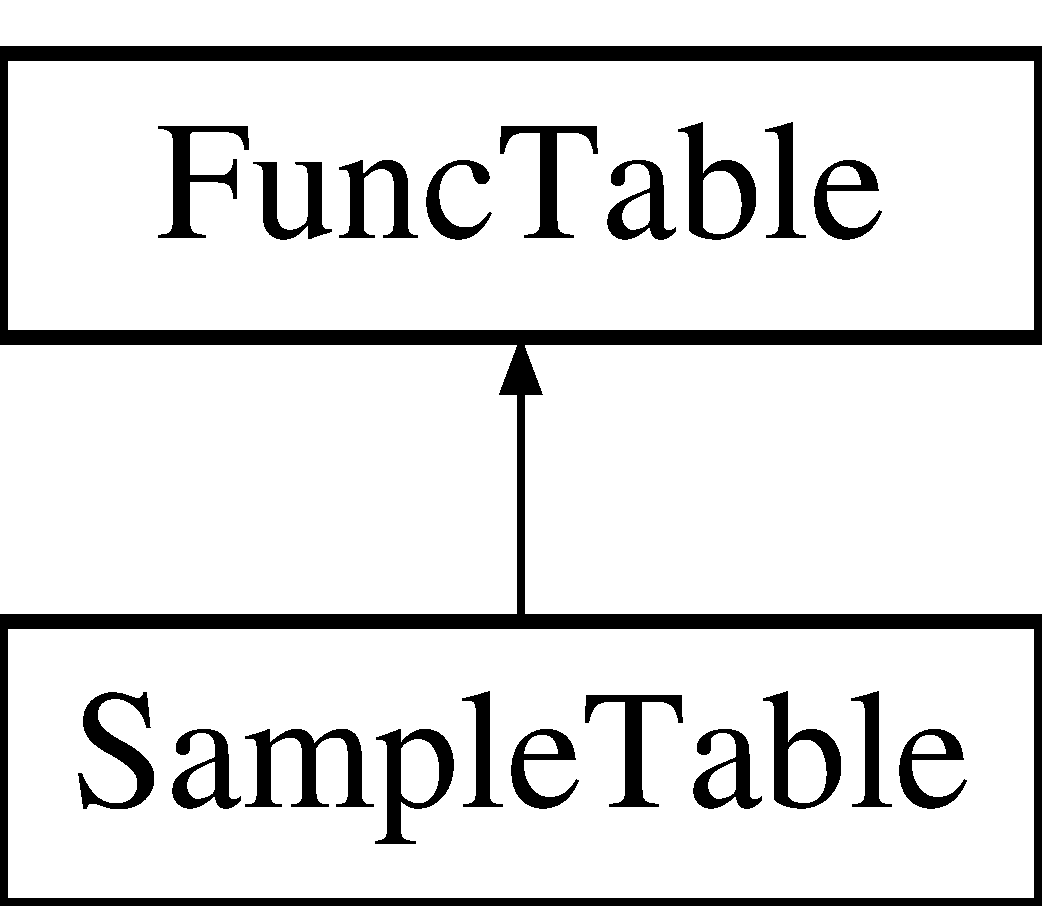
\includegraphics[height=2.000000cm]{class_sample_table}
\end{center}
\end{figure}
\subsection*{Public Member Functions}
\begin{DoxyCompactItemize}
\item 
\hyperlink{class_sample_table_aefe6f992664d4072ef6d521fcd87f2b8}{Sample\+Table} (const char $\ast$name, uint32\+\_\+t chn=1)
\item 
uint32\+\_\+t \hyperlink{class_sample_table_abab11cfefc24be1ad15a5fdbf9cd29dc}{nchnls} ()
\end{DoxyCompactItemize}
\subsection*{Additional Inherited Members}


\subsection{Detailed Description}
Sampled-\/sound table from a soundfile 

\subsection{Constructor \& Destructor Documentation}
\mbox{\Hypertarget{class_sample_table_aefe6f992664d4072ef6d521fcd87f2b8}\label{class_sample_table_aefe6f992664d4072ef6d521fcd87f2b8}} 
\index{Sample\+Table@{Sample\+Table}!Sample\+Table@{Sample\+Table}}
\index{Sample\+Table@{Sample\+Table}!Sample\+Table@{Sample\+Table}}
\subsubsection{\texorpdfstring{Sample\+Table()}{SampleTable()}}
{\footnotesize\ttfamily Sample\+Table\+::\+Sample\+Table (\begin{DoxyParamCaption}\item[{const char $\ast$}]{name,  }\item[{uint32\+\_\+t}]{chn = {\ttfamily 1} }\end{DoxyParamCaption})}

\hyperlink{class_sample_table}{Sample\+Table} constructor ~\newline
~\newline
name -\/ filename ~\newline
chn -\/ channel to load (0 = all channels) ~\newline


\subsection{Member Function Documentation}
\mbox{\Hypertarget{class_sample_table_abab11cfefc24be1ad15a5fdbf9cd29dc}\label{class_sample_table_abab11cfefc24be1ad15a5fdbf9cd29dc}} 
\index{Sample\+Table@{Sample\+Table}!nchnls@{nchnls}}
\index{nchnls@{nchnls}!Sample\+Table@{Sample\+Table}}
\subsubsection{\texorpdfstring{nchnls()}{nchnls()}}
{\footnotesize\ttfamily uint32\+\_\+t Sample\+Table\+::nchnls (\begin{DoxyParamCaption}{ }\end{DoxyParamCaption})\hspace{0.3cm}{\ttfamily [inline]}}

Get the number of channels 

The documentation for this class was generated from the following files\+:\begin{DoxyCompactItemize}
\item 
src/Sample\+Table.\+h\item 
src/Sample\+Table.\+cpp\end{DoxyCompactItemize}

\hypertarget{struct_saw_table}{}\section{Saw\+Table Struct Reference}
\label{struct_saw_table}\index{Saw\+Table@{Saw\+Table}}


{\ttfamily \#include $<$Wave\+Tables.\+h$>$}

Inheritance diagram for Saw\+Table\+:\begin{figure}[H]
\begin{center}
\leavevmode
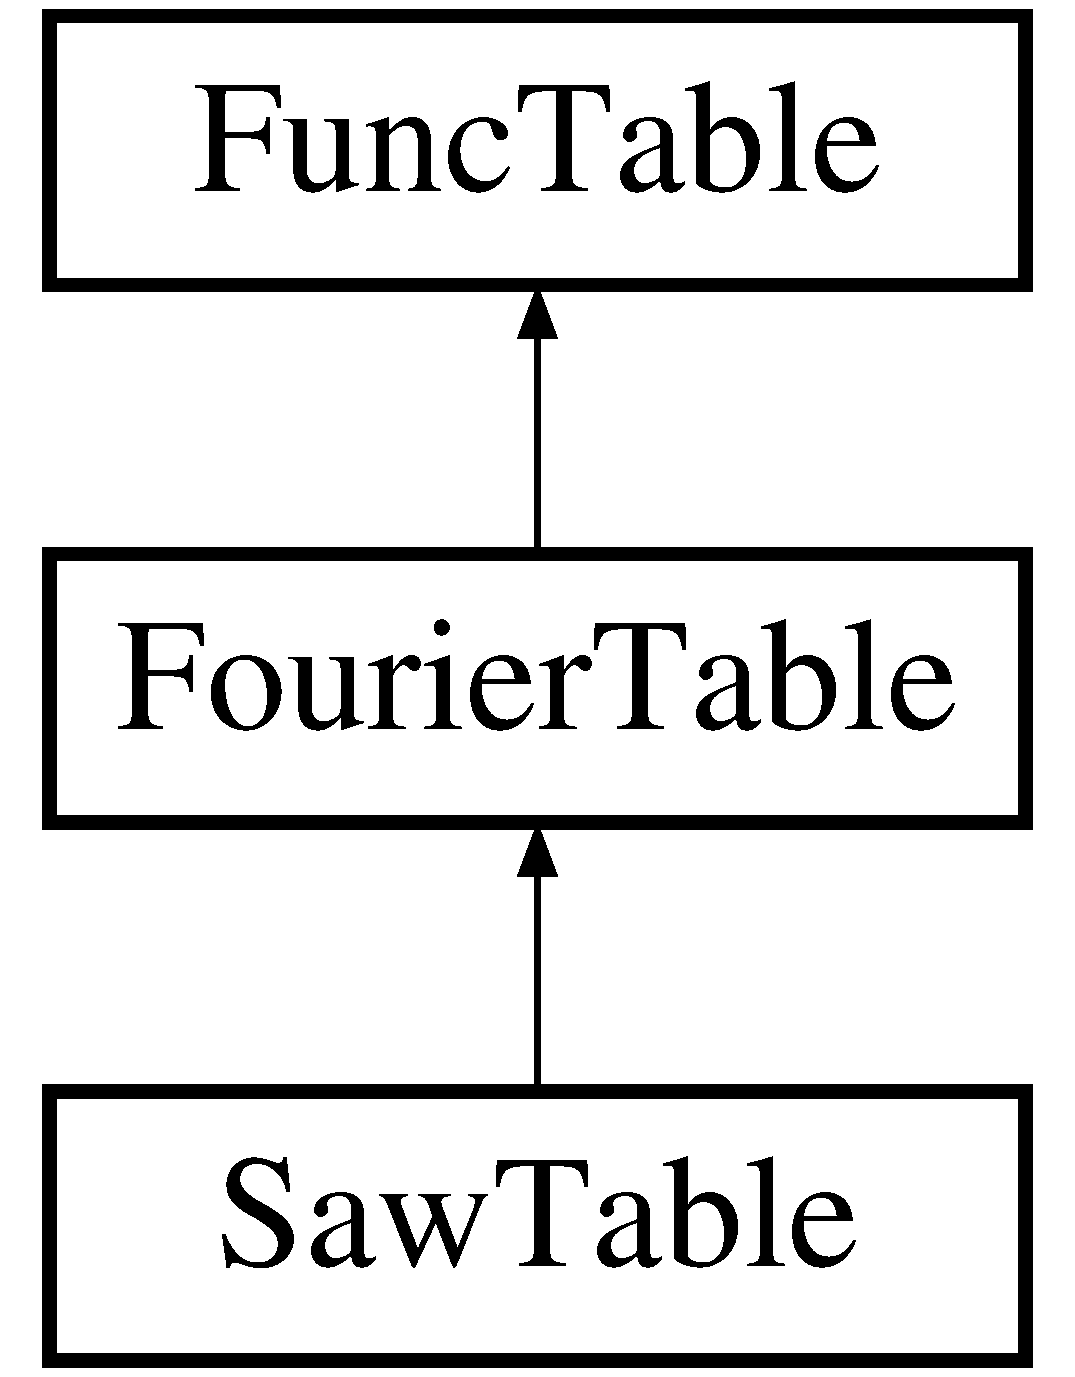
\includegraphics[height=3.000000cm]{struct_saw_table}
\end{center}
\end{figure}
\subsection*{Public Member Functions}
\begin{DoxyCompactItemize}
\item 
\hyperlink{struct_saw_table_a516fb9a4d13a31694fc820b2f326b6aa}{Saw\+Table} (uint32\+\_\+t harms, uint32\+\_\+t tsize=def\+\_\+tsize)
\end{DoxyCompactItemize}
\subsection*{Additional Inherited Members}


\subsection{Detailed Description}
Sawtooth wave table 

\subsection{Constructor \& Destructor Documentation}
\mbox{\Hypertarget{struct_saw_table_a516fb9a4d13a31694fc820b2f326b6aa}\label{struct_saw_table_a516fb9a4d13a31694fc820b2f326b6aa}} 
\index{Saw\+Table@{Saw\+Table}!Saw\+Table@{Saw\+Table}}
\index{Saw\+Table@{Saw\+Table}!Saw\+Table@{Saw\+Table}}
\subsubsection{\texorpdfstring{Saw\+Table()}{SawTable()}}
{\footnotesize\ttfamily Saw\+Table\+::\+Saw\+Table (\begin{DoxyParamCaption}\item[{uint32\+\_\+t}]{harms,  }\item[{uint32\+\_\+t}]{tsize = {\ttfamily def\+\_\+tsize} }\end{DoxyParamCaption})\hspace{0.3cm}{\ttfamily [inline]}}

\hyperlink{struct_saw_table}{Saw\+Table} constructor ~\newline
~\newline
harms -\/ number of harmonics ~\newline
tsize -\/ table size ~\newline


The documentation for this struct was generated from the following file\+:\begin{DoxyCompactItemize}
\item 
src/Wave\+Tables.\+h\end{DoxyCompactItemize}

\hypertarget{class_sound_in}{}\section{Sound\+In Class Reference}
\label{class_sound_in}\index{Sound\+In@{Sound\+In}}


{\ttfamily \#include $<$Sound\+In.\+h$>$}

Inheritance diagram for Sound\+In\+:\begin{figure}[H]
\begin{center}
\leavevmode
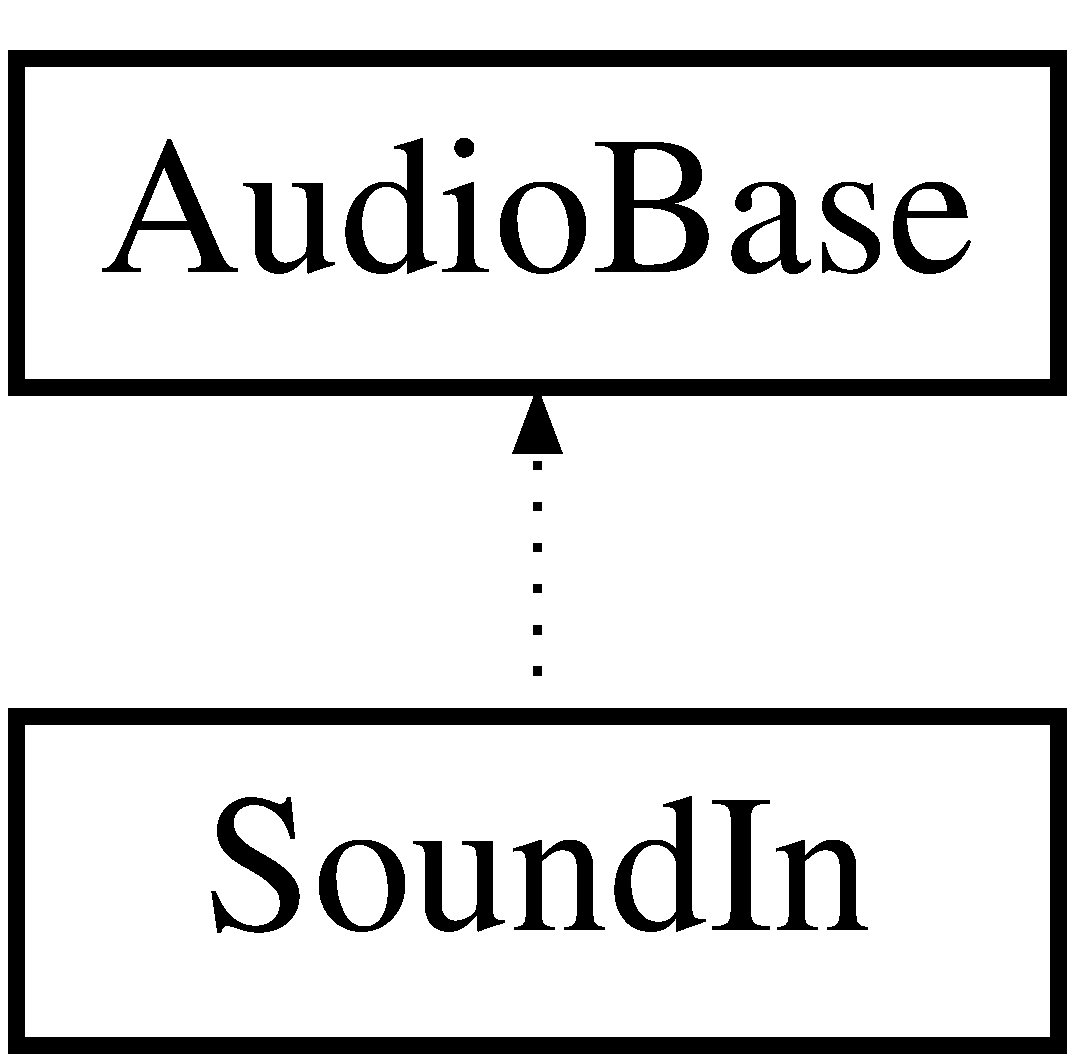
\includegraphics[height=2.000000cm]{class_sound_in}
\end{center}
\end{figure}
\subsection*{Public Member Functions}
\begin{DoxyCompactItemize}
\item 
\hyperlink{class_sound_in_a30492d30e5a18e2dda866a454779c210}{Sound\+In} (const char $\ast$src, uint32\+\_\+t vsize=def\+\_\+vsize, uint32\+\_\+t bsize=def\+\_\+bsize)
\item 
\hyperlink{class_sound_in_ac72a498714e161d1d691821f1214f2f3}{$\sim$\+Sound\+In} ()
\item 
uint32\+\_\+t \hyperlink{class_sound_in_adef1afd60041390537e1f3cef1e5a282}{read} ()
\end{DoxyCompactItemize}


\subsection{Detailed Description}
Audio input class 

\subsection{Constructor \& Destructor Documentation}
\mbox{\Hypertarget{class_sound_in_a30492d30e5a18e2dda866a454779c210}\label{class_sound_in_a30492d30e5a18e2dda866a454779c210}} 
\index{Sound\+In@{Sound\+In}!Sound\+In@{Sound\+In}}
\index{Sound\+In@{Sound\+In}!Sound\+In@{Sound\+In}}
\subsubsection{\texorpdfstring{Sound\+In()}{SoundIn()}}
{\footnotesize\ttfamily Sound\+In\+::\+Sound\+In (\begin{DoxyParamCaption}\item[{const char $\ast$}]{src,  }\item[{uint32\+\_\+t}]{vsize = {\ttfamily def\+\_\+vsize},  }\item[{uint32\+\_\+t}]{bsize = {\ttfamily def\+\_\+bsize} }\end{DoxyParamCaption})}

\hyperlink{class_sound_in}{Sound\+In} constructor ~\newline
~\newline
src -\/ input source (\char`\"{}adc\char`\"{}, \char`\"{}stdin\char`\"{}, or file path) ~\newline
vsize -\/ vector size ~\newline
bsize -\/ buffer size ~\newline
\mbox{\Hypertarget{class_sound_in_ac72a498714e161d1d691821f1214f2f3}\label{class_sound_in_ac72a498714e161d1d691821f1214f2f3}} 
\index{Sound\+In@{Sound\+In}!````~Sound\+In@{$\sim$\+Sound\+In}}
\index{````~Sound\+In@{$\sim$\+Sound\+In}!Sound\+In@{Sound\+In}}
\subsubsection{\texorpdfstring{$\sim$\+Sound\+In()}{~SoundIn()}}
{\footnotesize\ttfamily Sound\+In\+::$\sim$\+Sound\+In (\begin{DoxyParamCaption}{ }\end{DoxyParamCaption})}

\hyperlink{class_sound_out}{Sound\+Out} destructor 

\subsection{Member Function Documentation}
\mbox{\Hypertarget{class_sound_in_adef1afd60041390537e1f3cef1e5a282}\label{class_sound_in_adef1afd60041390537e1f3cef1e5a282}} 
\index{Sound\+In@{Sound\+In}!read@{read}}
\index{read@{read}!Sound\+In@{Sound\+In}}
\subsubsection{\texorpdfstring{read()}{read()}}
{\footnotesize\ttfamily uint32\+\_\+t Sound\+In\+::read (\begin{DoxyParamCaption}{ }\end{DoxyParamCaption})}

Reads audio into output vector 

The documentation for this class was generated from the following file\+:\begin{DoxyCompactItemize}
\item 
src/Sound\+In.\+h\end{DoxyCompactItemize}

\hypertarget{class_sound_out}{}\section{Sound\+Out Class Reference}
\label{class_sound_out}\index{Sound\+Out@{Sound\+Out}}


{\ttfamily \#include $<$Sound\+Out.\+h$>$}

\subsection*{Public Member Functions}
\begin{DoxyCompactItemize}
\item 
\hyperlink{class_sound_out_aaf7273b64d412247edff8264dc2b8f15}{Sound\+Out} (const char $\ast$dest, uint32\+\_\+t nchnls=def\+\_\+nchnls, double sr=def\+\_\+sr, uint32\+\_\+t vsize=def\+\_\+vsize, uint32\+\_\+t bsize=def\+\_\+bsize)
\item 
\hyperlink{class_sound_out_acef6789ce8fd42636630cd19287d23d6}{$\sim$\+Sound\+Out} ()
\item 
uint32\+\_\+t \hyperlink{class_sound_out_ae2cb2b2e4679a44c467e11f1893961f5}{write} (double $\ast$sig)
\end{DoxyCompactItemize}


\subsection{Detailed Description}
Generic audio output class 

\subsection{Constructor \& Destructor Documentation}
\mbox{\Hypertarget{class_sound_out_aaf7273b64d412247edff8264dc2b8f15}\label{class_sound_out_aaf7273b64d412247edff8264dc2b8f15}} 
\index{Sound\+Out@{Sound\+Out}!Sound\+Out@{Sound\+Out}}
\index{Sound\+Out@{Sound\+Out}!Sound\+Out@{Sound\+Out}}
\subsubsection{\texorpdfstring{Sound\+Out()}{SoundOut()}}
{\footnotesize\ttfamily Sound\+Out\+::\+Sound\+Out (\begin{DoxyParamCaption}\item[{const char $\ast$}]{dest,  }\item[{uint32\+\_\+t}]{nchnls = {\ttfamily def\+\_\+nchnls},  }\item[{double}]{sr = {\ttfamily def\+\_\+sr},  }\item[{uint32\+\_\+t}]{vsize = {\ttfamily def\+\_\+vsize},  }\item[{uint32\+\_\+t}]{bsize = {\ttfamily def\+\_\+bsize} }\end{DoxyParamCaption})}

\hyperlink{class_sound_out}{Sound\+Out} constructor ~\newline
~\newline
dest -\/ output destination (\char`\"{}dac\char`\"{}, \char`\"{}stdout\char`\"{}, or file path) ~\newline
nchnls -\/ number of channels ~\newline
sr -\/ sampling rate ~\newline
vsize -\/ vector size ~\newline
bsize -\/ buffer size ~\newline
\mbox{\Hypertarget{class_sound_out_acef6789ce8fd42636630cd19287d23d6}\label{class_sound_out_acef6789ce8fd42636630cd19287d23d6}} 
\index{Sound\+Out@{Sound\+Out}!````~Sound\+Out@{$\sim$\+Sound\+Out}}
\index{````~Sound\+Out@{$\sim$\+Sound\+Out}!Sound\+Out@{Sound\+Out}}
\subsubsection{\texorpdfstring{$\sim$\+Sound\+Out()}{~SoundOut()}}
{\footnotesize\ttfamily Sound\+Out\+::$\sim$\+Sound\+Out (\begin{DoxyParamCaption}{ }\end{DoxyParamCaption})}

\hyperlink{class_sound_out}{Sound\+Out} destructor 

\subsection{Member Function Documentation}
\mbox{\Hypertarget{class_sound_out_ae2cb2b2e4679a44c467e11f1893961f5}\label{class_sound_out_ae2cb2b2e4679a44c467e11f1893961f5}} 
\index{Sound\+Out@{Sound\+Out}!write@{write}}
\index{write@{write}!Sound\+Out@{Sound\+Out}}
\subsubsection{\texorpdfstring{write()}{write()}}
{\footnotesize\ttfamily uint32\+\_\+t Sound\+Out\+::write (\begin{DoxyParamCaption}\item[{double $\ast$}]{sig }\end{DoxyParamCaption})}

Writes sig to the output destination. 

The documentation for this class was generated from the following files\+:\begin{DoxyCompactItemize}
\item 
src/Sound\+Out.\+h\item 
src/Sound\+Out.\+cpp\end{DoxyCompactItemize}

\hypertarget{struct_square_table}{}\section{Square\+Table Struct Reference}
\label{struct_square_table}\index{Square\+Table@{Square\+Table}}


{\ttfamily \#include $<$Wave\+Tables.\+h$>$}

Inheritance diagram for Square\+Table\+:\begin{figure}[H]
\begin{center}
\leavevmode
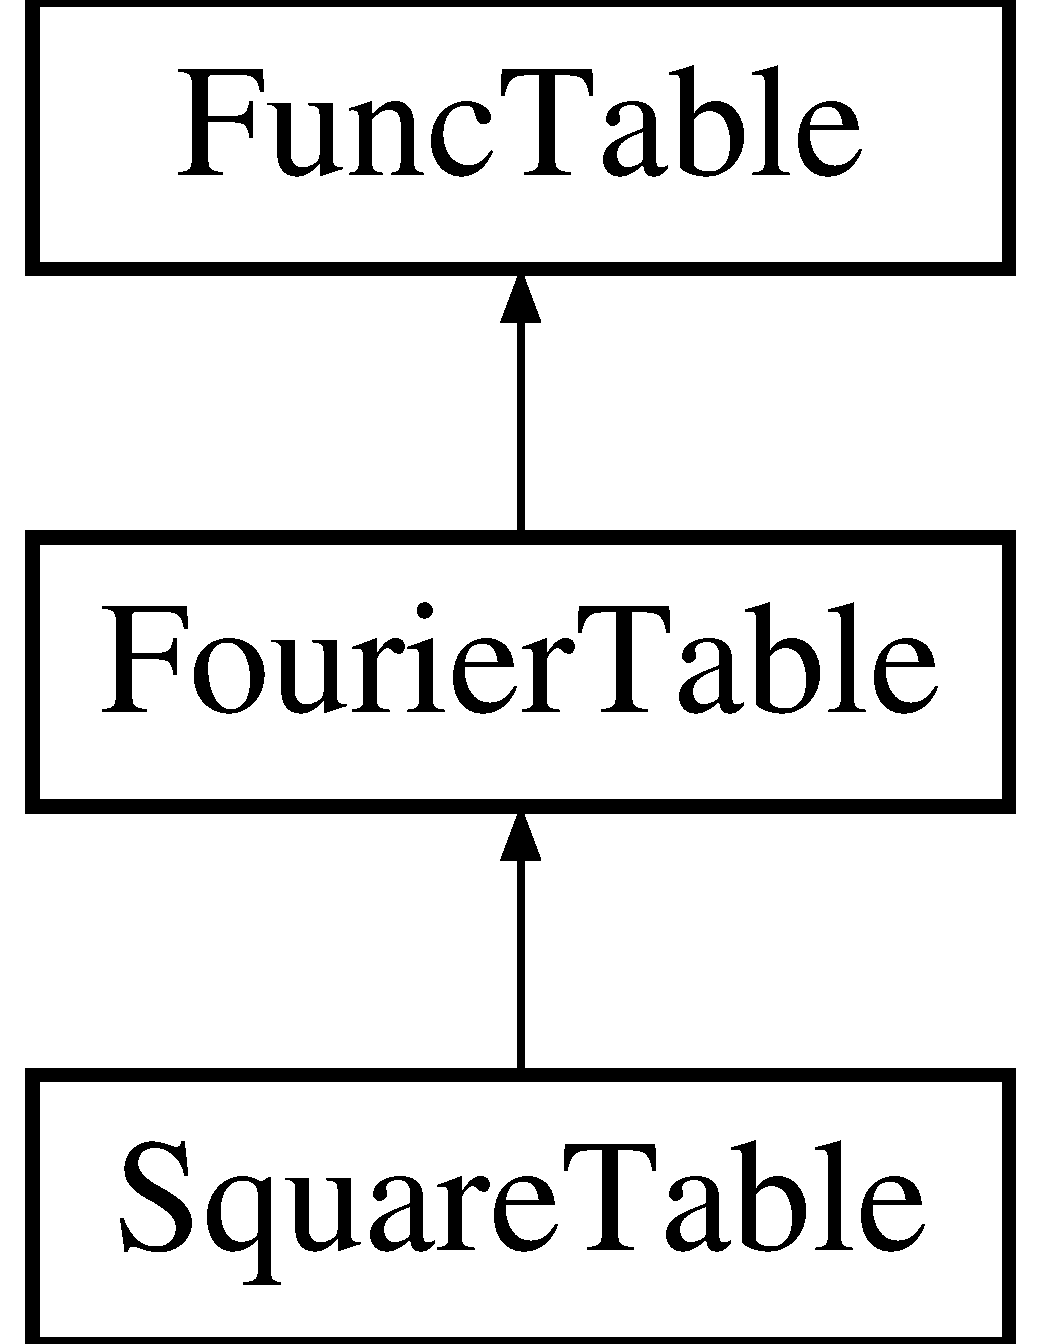
\includegraphics[height=3.000000cm]{struct_square_table}
\end{center}
\end{figure}
\subsection*{Public Member Functions}
\begin{DoxyCompactItemize}
\item 
\hyperlink{struct_square_table_a4bd437446f86b5440ca3b7e79785770d}{Square\+Table} (uint32\+\_\+t harms, uint32\+\_\+t tsize=def\+\_\+tsize)
\end{DoxyCompactItemize}
\subsection*{Additional Inherited Members}


\subsection{Detailed Description}
Square wave table 

\subsection{Constructor \& Destructor Documentation}
\mbox{\Hypertarget{struct_square_table_a4bd437446f86b5440ca3b7e79785770d}\label{struct_square_table_a4bd437446f86b5440ca3b7e79785770d}} 
\index{Square\+Table@{Square\+Table}!Square\+Table@{Square\+Table}}
\index{Square\+Table@{Square\+Table}!Square\+Table@{Square\+Table}}
\subsubsection{\texorpdfstring{Square\+Table()}{SquareTable()}}
{\footnotesize\ttfamily Square\+Table\+::\+Square\+Table (\begin{DoxyParamCaption}\item[{uint32\+\_\+t}]{harms,  }\item[{uint32\+\_\+t}]{tsize = {\ttfamily def\+\_\+tsize} }\end{DoxyParamCaption})\hspace{0.3cm}{\ttfamily [inline]}}

\hyperlink{struct_square_table}{Square\+Table} constructor ~\newline
~\newline
harms -\/ number of harmonics ~\newline
tsize -\/ table size ~\newline


The documentation for this struct was generated from the following file\+:\begin{DoxyCompactItemize}
\item 
src/Wave\+Tables.\+h\end{DoxyCompactItemize}

\hypertarget{class_table_read}{}\section{Table\+Read Class Reference}
\label{class_table_read}\index{Table\+Read@{Table\+Read}}


{\ttfamily \#include $<$Table\+Read.\+h$>$}

Inheritance diagram for Table\+Read\+:\begin{figure}[H]
\begin{center}
\leavevmode
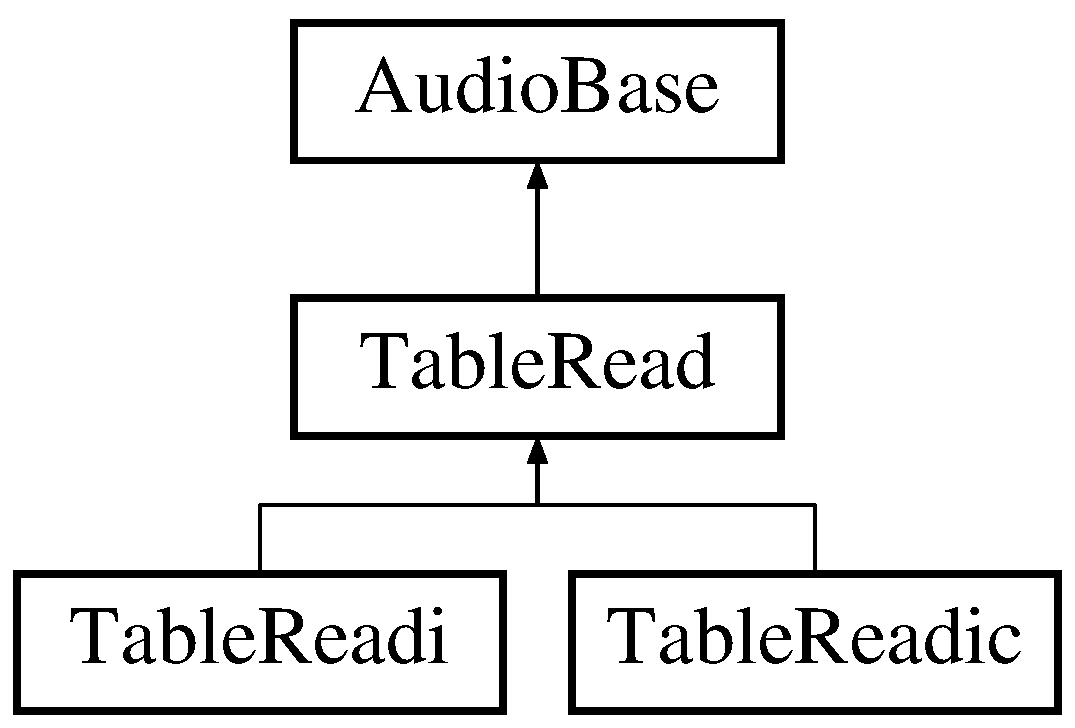
\includegraphics[height=3.000000cm]{class_table_read}
\end{center}
\end{figure}
\subsection*{Public Member Functions}
\begin{DoxyCompactItemize}
\item 
\hyperlink{class_table_read_a0ca6b6a46416b6ae1a48af6a490de9ff}{Table\+Read} (double $\ast$table, double phase=0., bool norm=true, bool wrap=true, uint32\+\_\+t tsize=def\+\_\+tsize, uint32\+\_\+t vsize=def\+\_\+vsize)
\item 
virtual void \hyperlink{class_table_read_ada219536a398309150f5f1270ac9534e}{process} (double $\ast$phs)
\end{DoxyCompactItemize}


\subsection{Detailed Description}
Table reader with truncated lookup 

\subsection{Constructor \& Destructor Documentation}
\mbox{\Hypertarget{class_table_read_a0ca6b6a46416b6ae1a48af6a490de9ff}\label{class_table_read_a0ca6b6a46416b6ae1a48af6a490de9ff}} 
\index{Table\+Read@{Table\+Read}!Table\+Read@{Table\+Read}}
\index{Table\+Read@{Table\+Read}!Table\+Read@{Table\+Read}}
\subsubsection{\texorpdfstring{Table\+Read()}{TableRead()}}
{\footnotesize\ttfamily Table\+Read\+::\+Table\+Read (\begin{DoxyParamCaption}\item[{double $\ast$}]{table,  }\item[{double}]{phase = {\ttfamily 0.},  }\item[{bool}]{norm = {\ttfamily true},  }\item[{bool}]{wrap = {\ttfamily true},  }\item[{uint32\+\_\+t}]{tsize = {\ttfamily def\+\_\+tsize},  }\item[{uint32\+\_\+t}]{vsize = {\ttfamily def\+\_\+vsize} }\end{DoxyParamCaption})\hspace{0.3cm}{\ttfamily [inline]}}

\hyperlink{class_table_read}{Table\+Read} constructor ~\newline
~\newline
table -\/ function table ~\newline
phase -\/ initial phase ~\newline
norm -\/ normalisation switch ~\newline
wrap -\/ wraparound switch ~\newline
tsize -\/ table size ~\newline
vsize -\/ vector size ~\newline


\subsection{Member Function Documentation}
\mbox{\Hypertarget{class_table_read_ada219536a398309150f5f1270ac9534e}\label{class_table_read_ada219536a398309150f5f1270ac9534e}} 
\index{Table\+Read@{Table\+Read}!process@{process}}
\index{process@{process}!Table\+Read@{Table\+Read}}
\subsubsection{\texorpdfstring{process()}{process()}}
{\footnotesize\ttfamily void Table\+Read\+::process (\begin{DoxyParamCaption}\item[{double $\ast$}]{phs }\end{DoxyParamCaption})\hspace{0.3cm}{\ttfamily [virtual]}}

takes in a frame of phase values and lookups up the table values 

Reimplemented in \hyperlink{class_table_readic_acc300e7cf5cf06af7d4aa06dde917f3c}{Table\+Readic}, and \hyperlink{class_table_readi_a636913b122affaa2b7bde68114f35a4a}{Table\+Readi}.



The documentation for this class was generated from the following files\+:\begin{DoxyCompactItemize}
\item 
src/Table\+Read.\+h\item 
src/Table\+Read.\+cpp\end{DoxyCompactItemize}

\hypertarget{class_table_readi}{}\section{Table\+Readi Class Reference}
\label{class_table_readi}\index{Table\+Readi@{Table\+Readi}}


{\ttfamily \#include $<$Table\+Readi.\+h$>$}

Inheritance diagram for Table\+Readi\+:\begin{figure}[H]
\begin{center}
\leavevmode
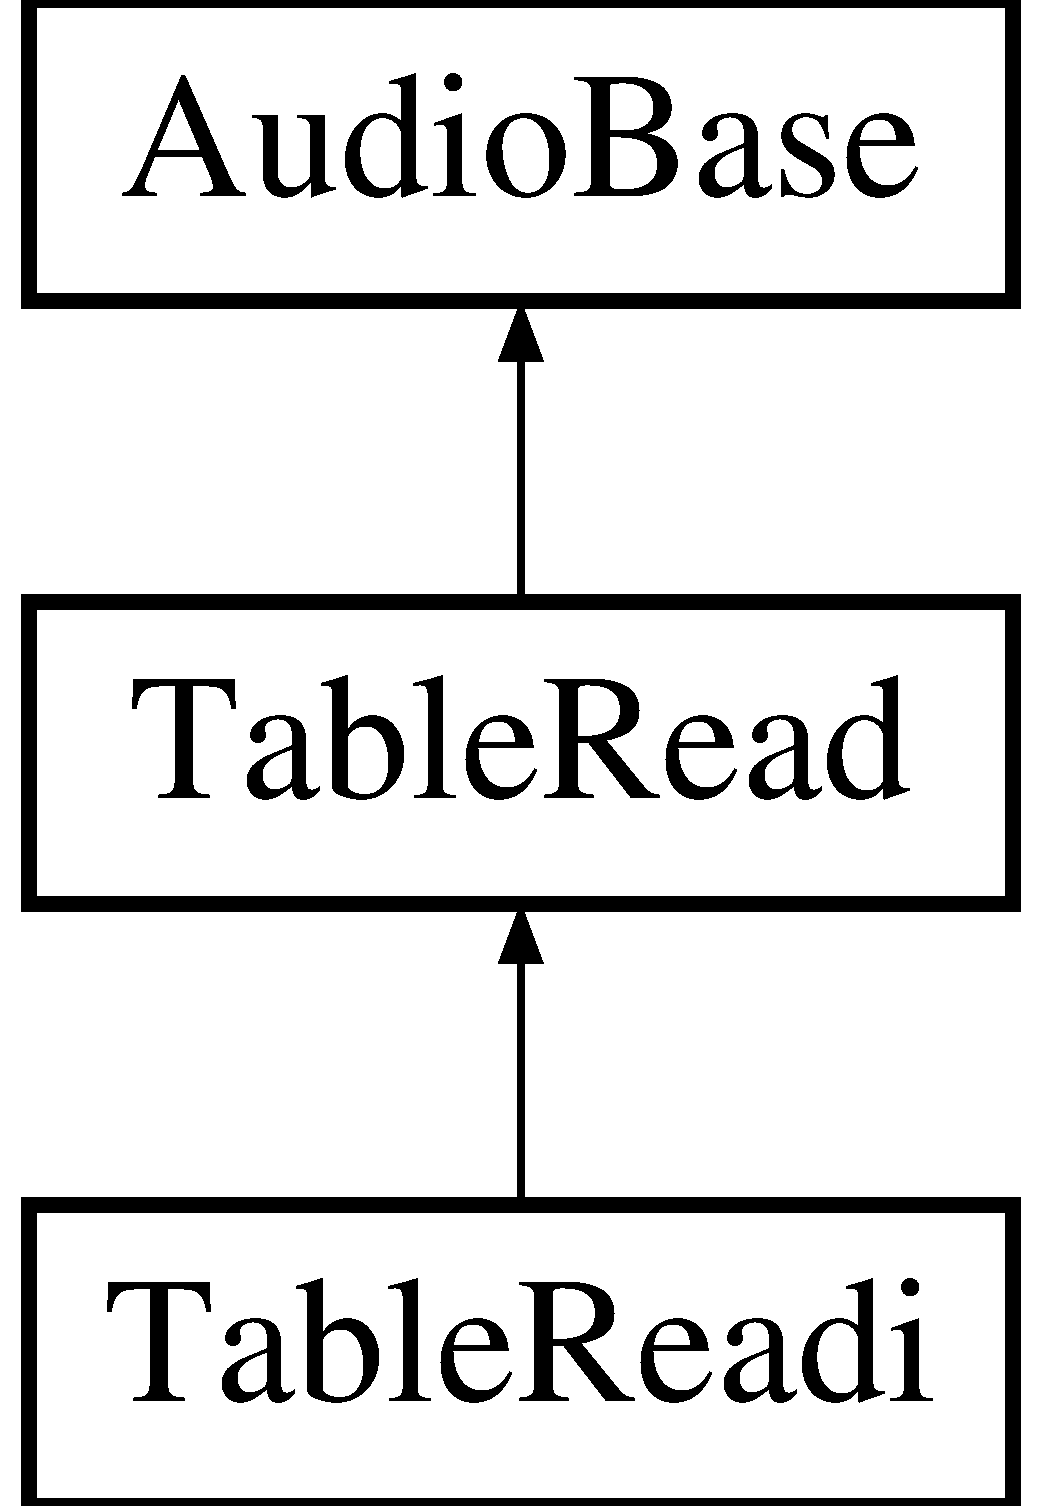
\includegraphics[height=3.000000cm]{class_table_readi}
\end{center}
\end{figure}
\subsection*{Public Member Functions}
\begin{DoxyCompactItemize}
\item 
\hyperlink{class_table_readi_aa5e834103bbeb0ea48982ec10c2c0e9a}{Table\+Readi} (double $\ast$table, double phase=0., bool norm=true, bool wrap=true, uint32\+\_\+t tsize=def\+\_\+tsize, uint32\+\_\+t vsize=def\+\_\+vsize)
\item 
virtual void \hyperlink{class_table_readi_a636913b122affaa2b7bde68114f35a4a}{process} (double $\ast$phs)
\end{DoxyCompactItemize}


\subsection{Detailed Description}
Table reader with linear interpolation 

\subsection{Constructor \& Destructor Documentation}
\mbox{\Hypertarget{class_table_readi_aa5e834103bbeb0ea48982ec10c2c0e9a}\label{class_table_readi_aa5e834103bbeb0ea48982ec10c2c0e9a}} 
\index{Table\+Readi@{Table\+Readi}!Table\+Readi@{Table\+Readi}}
\index{Table\+Readi@{Table\+Readi}!Table\+Readi@{Table\+Readi}}
\subsubsection{\texorpdfstring{Table\+Readi()}{TableReadi()}}
{\footnotesize\ttfamily Table\+Readi\+::\+Table\+Readi (\begin{DoxyParamCaption}\item[{double $\ast$}]{table,  }\item[{double}]{phase = {\ttfamily 0.},  }\item[{bool}]{norm = {\ttfamily true},  }\item[{bool}]{wrap = {\ttfamily true},  }\item[{uint32\+\_\+t}]{tsize = {\ttfamily def\+\_\+tsize},  }\item[{uint32\+\_\+t}]{vsize = {\ttfamily def\+\_\+vsize} }\end{DoxyParamCaption})\hspace{0.3cm}{\ttfamily [inline]}}

\hyperlink{class_table_readi}{Table\+Readi} constructor ~\newline
~\newline
table -\/ function table ~\newline
phase -\/ initial phase ~\newline
norm -\/ normalisation switch ~\newline
wrap -\/ wraparound switch ~\newline
tsize -\/ table size ~\newline
vsize -\/ vector size ~\newline


\subsection{Member Function Documentation}
\mbox{\Hypertarget{class_table_readi_a636913b122affaa2b7bde68114f35a4a}\label{class_table_readi_a636913b122affaa2b7bde68114f35a4a}} 
\index{Table\+Readi@{Table\+Readi}!process@{process}}
\index{process@{process}!Table\+Readi@{Table\+Readi}}
\subsubsection{\texorpdfstring{process()}{process()}}
{\footnotesize\ttfamily void Table\+Readi\+::process (\begin{DoxyParamCaption}\item[{double $\ast$}]{phs }\end{DoxyParamCaption})\hspace{0.3cm}{\ttfamily [virtual]}}

takes in a frame of phase values and lookups up the table values 

Reimplemented from \hyperlink{class_table_read_ada219536a398309150f5f1270ac9534e}{Table\+Read}.



The documentation for this class was generated from the following files\+:\begin{DoxyCompactItemize}
\item 
src/Table\+Readi.\+h\item 
src/Table\+Readi.\+cpp\end{DoxyCompactItemize}

\hypertarget{class_table_readic}{}\section{Table\+Readic Class Reference}
\label{class_table_readic}\index{Table\+Readic@{Table\+Readic}}


{\ttfamily \#include $<$Table\+Readic.\+h$>$}

Inheritance diagram for Table\+Readic\+:\begin{figure}[H]
\begin{center}
\leavevmode
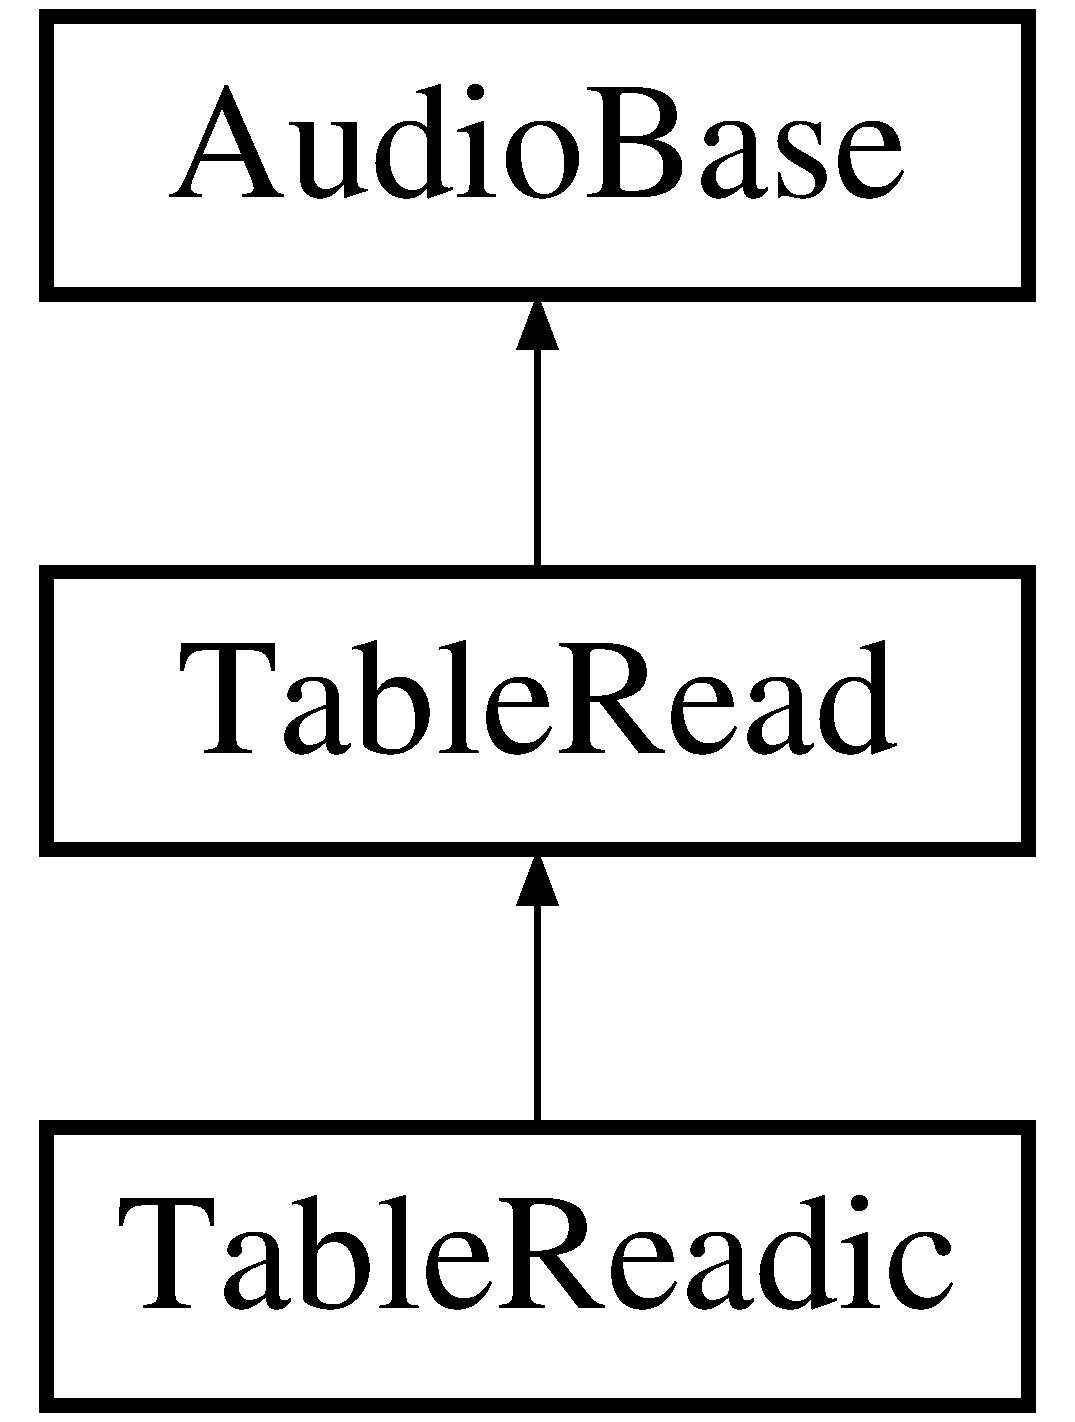
\includegraphics[height=3.000000cm]{class_table_readic}
\end{center}
\end{figure}
\subsection*{Public Member Functions}
\begin{DoxyCompactItemize}
\item 
\hyperlink{class_table_readic_a792cbe0b54c4adf39a9000f4ac3f7513}{Table\+Readic} (double $\ast$table, double phase=0., bool norm=true, bool wrap=true, uint32\+\_\+t tsize=def\+\_\+tsize, uint32\+\_\+t vsize=def\+\_\+vsize)
\item 
virtual void \hyperlink{class_table_readic_acc300e7cf5cf06af7d4aa06dde917f3c}{process} (double $\ast$phs)
\end{DoxyCompactItemize}


\subsection{Detailed Description}
Table reader with cubic interpolation 

\subsection{Constructor \& Destructor Documentation}
\mbox{\Hypertarget{class_table_readic_a792cbe0b54c4adf39a9000f4ac3f7513}\label{class_table_readic_a792cbe0b54c4adf39a9000f4ac3f7513}} 
\index{Table\+Readic@{Table\+Readic}!Table\+Readic@{Table\+Readic}}
\index{Table\+Readic@{Table\+Readic}!Table\+Readic@{Table\+Readic}}
\subsubsection{\texorpdfstring{Table\+Readic()}{TableReadic()}}
{\footnotesize\ttfamily Table\+Readic\+::\+Table\+Readic (\begin{DoxyParamCaption}\item[{double $\ast$}]{table,  }\item[{double}]{phase = {\ttfamily 0.},  }\item[{bool}]{norm = {\ttfamily true},  }\item[{bool}]{wrap = {\ttfamily true},  }\item[{uint32\+\_\+t}]{tsize = {\ttfamily def\+\_\+tsize},  }\item[{uint32\+\_\+t}]{vsize = {\ttfamily def\+\_\+vsize} }\end{DoxyParamCaption})\hspace{0.3cm}{\ttfamily [inline]}}

\hyperlink{class_table_readic}{Table\+Readic} constructor ~\newline
~\newline
table -\/ function table ~\newline
phase -\/ initial phase ~\newline
norm -\/ normalisation switch ~\newline
wrap -\/ wraparound switch ~\newline
tsize -\/ table size ~\newline
vsize -\/ vector size ~\newline


\subsection{Member Function Documentation}
\mbox{\Hypertarget{class_table_readic_acc300e7cf5cf06af7d4aa06dde917f3c}\label{class_table_readic_acc300e7cf5cf06af7d4aa06dde917f3c}} 
\index{Table\+Readic@{Table\+Readic}!process@{process}}
\index{process@{process}!Table\+Readic@{Table\+Readic}}
\subsubsection{\texorpdfstring{process()}{process()}}
{\footnotesize\ttfamily void Table\+Readic\+::process (\begin{DoxyParamCaption}\item[{double $\ast$}]{phs }\end{DoxyParamCaption})\hspace{0.3cm}{\ttfamily [virtual]}}

takes in a frame of phase values and lookups up the table values 

Reimplemented from \hyperlink{class_table_read_ada219536a398309150f5f1270ac9534e}{Table\+Read}.



The documentation for this class was generated from the following files\+:\begin{DoxyCompactItemize}
\item 
src/Table\+Readic.\+h\item 
src/Table\+Readic.\+cpp\end{DoxyCompactItemize}

\hypertarget{struct_triangle_table}{}\section{Triangle\+Table Struct Reference}
\label{struct_triangle_table}\index{Triangle\+Table@{Triangle\+Table}}


{\ttfamily \#include $<$Wave\+Tables.\+h$>$}

Inheritance diagram for Triangle\+Table\+:\begin{figure}[H]
\begin{center}
\leavevmode
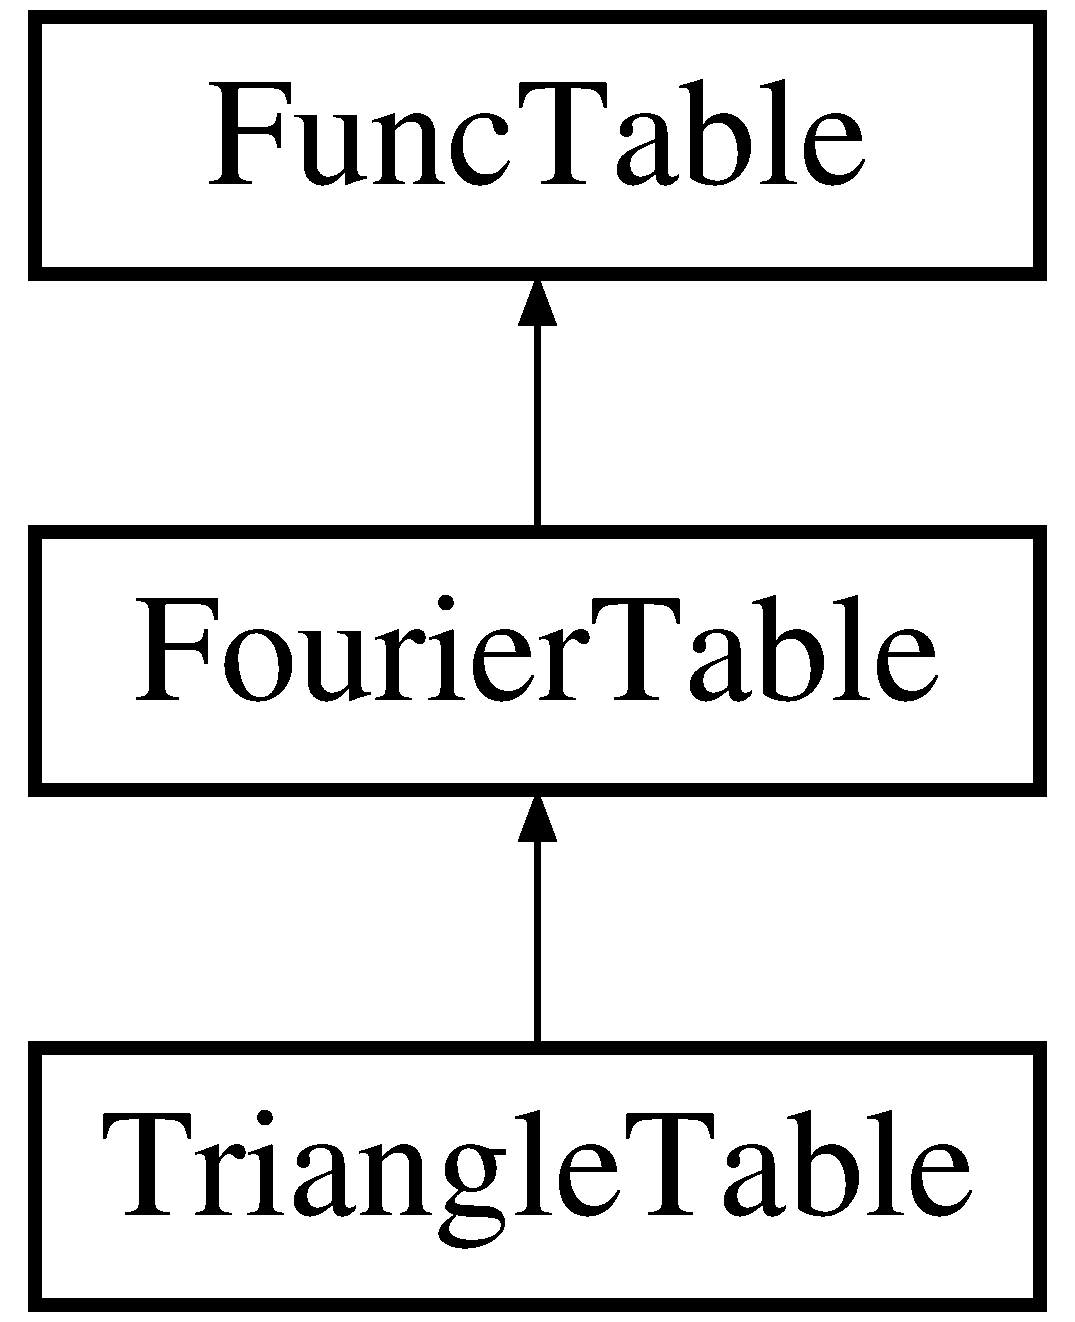
\includegraphics[height=3.000000cm]{struct_triangle_table}
\end{center}
\end{figure}
\subsection*{Public Member Functions}
\begin{DoxyCompactItemize}
\item 
\hyperlink{struct_triangle_table_a26a2345f91109060172b796ff9785299}{Triangle\+Table} (uint32\+\_\+t harms, uint32\+\_\+t tsize=def\+\_\+tsize)
\end{DoxyCompactItemize}
\subsection*{Additional Inherited Members}


\subsection{Detailed Description}
Triangle wave table 

\subsection{Constructor \& Destructor Documentation}
\mbox{\Hypertarget{struct_triangle_table_a26a2345f91109060172b796ff9785299}\label{struct_triangle_table_a26a2345f91109060172b796ff9785299}} 
\index{Triangle\+Table@{Triangle\+Table}!Triangle\+Table@{Triangle\+Table}}
\index{Triangle\+Table@{Triangle\+Table}!Triangle\+Table@{Triangle\+Table}}
\subsubsection{\texorpdfstring{Triangle\+Table()}{TriangleTable()}}
{\footnotesize\ttfamily Triangle\+Table\+::\+Triangle\+Table (\begin{DoxyParamCaption}\item[{uint32\+\_\+t}]{harms,  }\item[{uint32\+\_\+t}]{tsize = {\ttfamily def\+\_\+tsize} }\end{DoxyParamCaption})\hspace{0.3cm}{\ttfamily [inline]}}

\hyperlink{struct_triangle_table}{Triangle\+Table} constructor ~\newline
~\newline
harms -\/ number of harmonics ~\newline
tsize -\/ table size ~\newline


The documentation for this struct was generated from the following file\+:\begin{DoxyCompactItemize}
\item 
src/Wave\+Tables.\+h\end{DoxyCompactItemize}

%--- End generated contents ---

% Index
\backmatter
\newpage
\phantomsection
\clearemptydoublepage
\addcontentsline{toc}{chapter}{Index}
\printindex

\end{document}
